\documentclass[12pt,oneside]{book}
\usepackage{setspace}
\usepackage{amssymb}
\usepackage{amsmath}
\usepackage{mathtools}
\usepackage{graphicx}
\usepackage{textcomp}
\usepackage{xparse}
\usepackage{multirow}
\usepackage{caption}
\usepackage{subcaption}
\usepackage{titling}
\usepackage{algorithm}
\usepackage{algorithmicx}
\usepackage{algpseudocode}
\usepackage{titling}
\usepackage{url}
\graphicspath{ {./images/} }
\usepackage[utf8]{inputenc}
\usepackage[letterpaper,left=1.5in,right=1in,top=1in,bottom=1in]{geometry}
\DeclareMathOperator*{\argmin}{arg\,min}
\DeclareMathOperator*{\R}{\mathbb{R}}
\DeclareDocumentCommand{\E}{s m}{
  \operatorname{E}%
  \IfBooleanTF{#1}% Condition on *
    {#2}% Print only the argument in starred * version
    {\left[#2\right]}% Print bracketed argument [ ] in unstarred version
}
\newenvironment{definition}[1][Definition.]{\begin{trivlist}                         
  \item[\hskip \labelsep {\bfseries #1}]}{\end{trivlist}}
\setcounter{MaxMatrixCols}{20}
\begin{document}
\bibliographystyle{IEEEtran}
\pagenumbering{gobble}
{
\centering
\large\bf
THE COOPER UNION\\
ALBERT NERKEN SCHOOL OF ENGINEERING
\Large
\vskip 88pt
Crafting Adversarial Text Samples for Recurrent Neural Networks Using Windowed Inference and Search
\vskip 88pt
by\\
Cory Nezin
\vskip 88pt
A thesis submitted in partial fulfillment\\
of the requirements for the degree of\\
Master of Engineering
\vskip 88pt
May 2016
\vskip 88pt
Professor Fred L. Fontaine, Advisor

}

{
\large\bf
\begin{centering}
THE COOPER UNION FOR \\THE ADVANCEMENT OF SCIENCE AND ART\\
\vskip 36pt
ALBERT NERKEN SCHOOL OF ENGINEERING\\
\end{centering}
\vskip 88pt
\noindent
This thesis was prepared under the direction of the Candidate's Thesis Advisor
and has received approval. It was submitted to the Dean of the School of
Engineering and the full Faculty, and was approved as partial fulfillment of the
requirements for the degree of Master of Engineering.\\

\vskip 60pt

\normalsize
\hfill
\begin{tabular}{@{}p{.5in}p{3.8in}@{}}
&\hrulefill \\
& Richard Stock, Dean of Engineering \hskip 30pt Date
\end{tabular}

\vskip 60pt

\hspace*{-2.5cm}
\begin{tabular}{@{}p{.5in}p{3in}@{}}
& \hrulefill \\
& Professor Fred L. Fontaine \hskip 30pt Date \\
\end{tabular}\hfill

}

\frontmatter
\pagenumbering{roman}
{
\centering
\section*{Acknowledgments}
}
\doublespacing
\noindent
First and foremost I thank my advisor, Professor Fred Fontaine.  Professor Fontaine has served as an excellent adviser in all my time as an electrical engineering student.  He has shown fierce dedication to his field, The Cooper Union, and his students.  His signal processing course allowed me to discover a vast and interesting field, and he inspired me to pursue it.  This thesis would not be possible without his advisement and education which he provided me over the past two years.  I will not soon forget what I learned in his courses, nor the opportunities afforded as a result. \\

\noindent
I would like to thank all of my peers, the faculty, the alumni, the administration, and The Cooper Union as a whole.  This is a weird, beautiful, and sometimes pain inducing institution.  I feel that the sense of community is perhaps greater than any other place.  I hope that I will continue to be a part of the community for a long time so I can give back what The Cooper Union has given to me.  I give particular thanks to Brenda So, Ross Kaplan, and Gordon Macshane, some of the closest friends I made here.  They have helped me in ways I cannot even describe.\\

\noindent
Finally, I thank my parents.  They have always provided me support, and allowed me to grow to be my own person.  My intense work has reduced the time that I can spend with them, but I know they understand that this sacrifice is worth it. 

\doublespacing
\begin{abstract}
Neural networks have recently been found vulnerable to ``attacks'' which cause them to misclassify samples given a very small disturbance.  Attacks based on iterative gradient methods have been largely studied for continous domain samples like images.  In this work we introduce a hybrid algorithm for the non-continous domain of text.  Our algorithm uses gradient as a guide for candidate word replacements, and then performs an exponential search to determine the minimum number of replacements required to alter the classification of a text sample.  We test the algorithm under white box, gray box, and black box scenarios
\end{abstract}

\tableofcontents
\listoffigures
\listoftables
\mainmatter
\chapter{Introduction}
\section{Problem Statement}
Automatic text analysis and classification have become important issues with the rise of the internet and digital text.  Every minute, millions of emails and texts are sent, and at least thousands of news articles are published. \cite{jj17,mr16}.  With this huge rise in information, tools have been deployed to protect people from malicious actors. 

Spam emails are not only annoying but dangerous.  They often contain phishing scams which attempt to obtain identifying credentials from targets, or links to malicious software.  In 2002, a very effective email spam filter was developed which outperformed competitors by a large margin. \cite{bl02} The success of the algorithm was afforded by the implementation of Bayesian filtering.  The inventor of the algorithm, Paul Graham, applied basic rules of probability to the problem of classifying an email as spam or not.  Both spam filters and spam sources have of course evolved since then, both constantly attempting to overcome the other.

The term ``fake news'' which has recently come into existence.  Fake news refers to a news article which is intentionally created to misguide the readers with false statements.  With the new-found ease of creating a website that looks like a legitimate newspaper, it can be difficult to tell whether a news article is real or not.  The authors of \cite{nr17} suggest a machine learning solution, where an algorithm automatically separates fake news from true.

The huge rise of digital communication has also led to the expansion of forensic linguistics.  Automatic web scraping and search engine reporting can help investigative authorities identify criminals and terrorists on the internet.  Because of the huge amount of data to sift through, it is unlikely that the vast majority of text is analyzed by humans.  While organizations like the NSA, FBI, and, CIA are rightfully secretive about their methods, it is likely that they use some kind of pattern recognition or machine learning to identify suspicious individuals and organizations.

Recently, machine learning algorithms have been found vulnerable to adversarial attacks which cause them to misclassify samples after only minor alterations. \cite{cs14} While these adversarial attacks originally targeting image classifiers, they have been extended, to some extent, to the domain of language. \cite{np16} These attacks stand to compromise the methods of defense just previously described.  Neural networks in particular have been found extremely useful in those defenses, but also very vulnerable to adversarial attacks.  This thesis takes the perspective of the red team, and attempts to find efficient and effective methods of attack so that defenses may be correspondingly developed.

\section{Our Contribution}
This thesis contributes two algorithms for causing misclassification in recurrent neural networks acting on text.  The method found in \cite{np16} was an iterative method completely based on the gradient of the network with respect to the inputs.  This thesis finds the information provided by the gradient to unreliable, and describes search based methods instead.  One method, window search, does not even require a differentiable model.  The other method, gradient assisted window search, is a hybrid model which uses the gradient to search more quickly, though with degraded results.  

This work measures the performance of adversarial algorithms by counting the number of word replacements that are required to cause a misclassification.  Time to obtain a misclassification was also measured.  Both window search and gradient assisted window search show a very large improvement over the algorithm in \cite{np16} in a white box scenario, and an even larger improvement in a black box scenario.

\section{Overview}
Chapter 2 provides a background on machine learning, especially the algorithms employed in the experiments.  These algorithms include recurrently neural networks, word2vec, and gradient based training algorithms like gradient descent.  Chapter 3 describes the problem statement in more detail and develops the terminology and definitions to discuss it.  Chapter 4 briefly discusses the results obtained from training recurrent neural networks and a word embedding.  It also provides motivation for reducing the impact of the gradient on decision making in the algorithms.  Chapter 5 describes the developed algorithms in detail, and provides a time and space complexity analysis.  Chapter 6 gives a discussion of the results under several different scenarios.  Chapter 7 concludes the thesis with a summary of results and methods, as well as a discussion of future work.

\chapter{Background}
\section{Machine Learning}
\label{sec:machine_learning}
Machine learning is the general task of finding patterns given a set of data.  The methods by which these tasks are accomplished range from the simple linear regression to more complex neural networks.  Machine learning problems fall into primarily two categories: supervised learning and unsupervised learning.  

In the case of supervised learning, one is given a set of inputs, $\{x\}_{i=1}^N\in X$ and outputs, $\{y\}_{i=1}^N\in Y$ to some unknown function, $f$.  These sets are often referred to as ``features'' and ``labels'' respectively.  The goal is then to determine what that function is.  This is usually not feasible due the model for the function not being complex enough, or for being too complex.  These issues are known as underfitting and overfitting, respectively.  The objective is therefore simplified as finding the function, $g \in M$ where $M$ is some set of model functions, and where $g$ minimizes some loss function, $L(g,x,y)$.  That is:
\begin{align}
\argmin_{g \in M} L(g,x,y)
\end{align}

One simple case of this is linear regression.  In linear regression, $M$ is the set of linear (or in most cases affine) functions mapping $X$ to $Y$. and the loss function is $L(g,x,y) = \frac{1}{N} \sum_{i=1}^N ||g(x_i)-y_i||^2$  It turns out that under these constraints, an exact solution can be found.  An illustration where $X=Y= \mathbb{R}$ is shown in figure \ref{fig:linear_regression}.

\begin{figure}
    \centering
    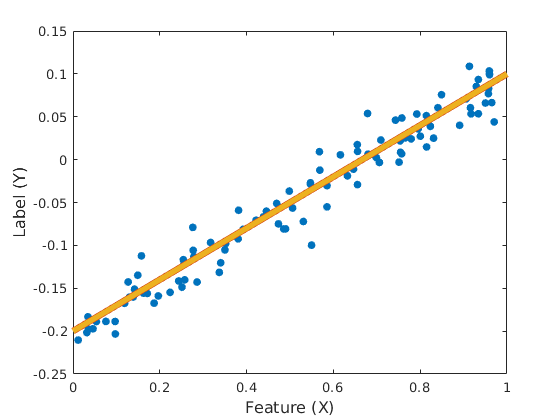
\includegraphics[width=0.8\textwidth]{linear_regression.png}
    \caption{Linear regression for a noisy line.  A blue dot represents the position of a feature/label pair.  The yellow line represents the approximate affine approximation function.}
    \label{fig:linear_regression}
\end{figure}

In the case of unsupervised learning, one is given only some set of features, $\{x\}_{i=1}^N$ and asked to find some pattern in the data.  Finding a pattern can consist of finding clusters of data points which are ``close'' together by some measure, or finding some lower dimensional representation for the data, these are essentially problems of lossy compression.  Usually algorithms work by minimizing some loss function so that techniques can be borrowed from supervised learning, though these are not necessarily measures of the algorithm's success.  

One well known example of unsupervised learning is principal component analysis and its cousin singular value decomposition.  Given some features in the form of a matrix $X$, singular value decomposition can be used to find a matrix, $\hat{X}$ of rank $r < rank(X)$ such that $||X-\hat{X}||_F$ is minimized.  This has the effect of finding a lower dimensional representation of $X$ which contains as much information as possible and therefore tells us which dimensions are ``important.''  One example is shown in figure \ref{fig:svd_recover} uses singular value decomposition to remove noise from an assumed low rank matrix.  In figure \ref{fig:singval_good}, a plot shows the relative contribution of automatically detected signal components.  

\begin{figure}
    \centering
    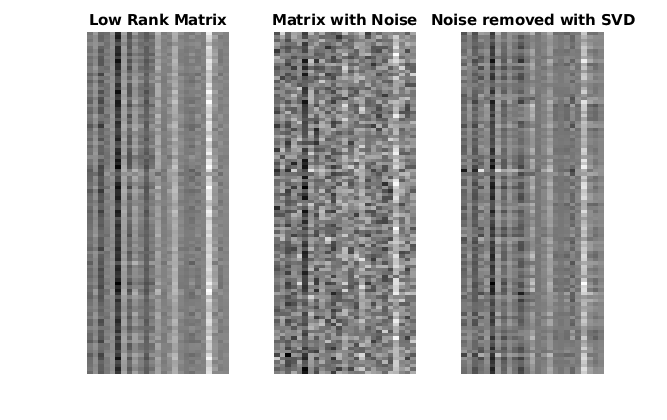
\includegraphics[width=0.8\textwidth]{svd_plots.png}
    \caption{Illustration of using SVD to recover an underlying signal.  This is an example of unsupervised learning.}
    \label{fig:svd_recover}
\end{figure}
\begin{figure}
    \centering
    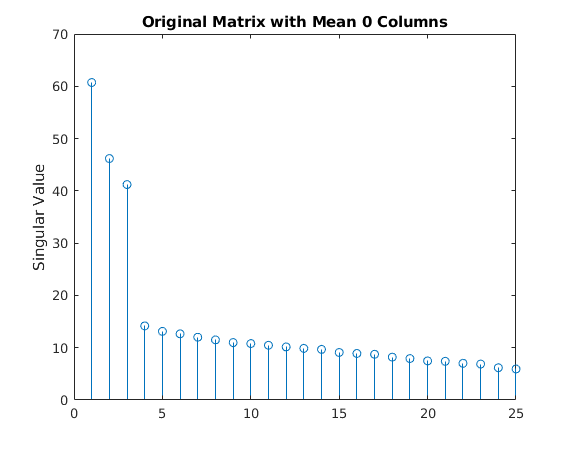
\includegraphics[width=0.8\textwidth]{singval0.png}
    \caption{Set of 25 singular value for the low rank matrix in figure \ref{fig:svd_recover}.  There are three distinct large values which tells us that the origin rank was very likely three.}
    \label{fig:singval_good}
\end{figure}

\subsection{Hyperparameters} \label{sec:hyperparameters}
Hyperparameters are parameters of a function which do not change during the ``learning process'', that is, they are set by the user at the beginning, and the regular parameters of the function are determined with the hyperparameters held constant.  In the example of using singular value decomposition to denoise a low rank matrix, the hyperparameter would be the desired rank of the resulting matrix.  

It can be seen from figure \ref{fig:singval_good} that this hyperparameter could be calculated, or at least guessed from the number of dominant singular values.  In most modern machine learning models, it is very difficult to efficiently determine optimal hyperparameters, often requiring a brute force search over several combinations.  This technique is known as grid search, which searches over $n$ hyperparameters on an $n$ dimensional grid and chooses the hyperparameters that minimize some loss function, not necessarily the same as the model's loss function.  The process of choosing optimal hyperparameters is known as hyperparameter tuning.

\subsection{Overfitting} \label{sec:overfitting}
If one allows the model, or set of permissible functions, to be more complex, one may represent more complicated functions.  Figure \ref{fig:poly_reg} shows an example of both a quadratic fit and a $20^{th}$ order polynomial fit to data points with a more complicated pattern.  These two images represent the issue of overfitting: while the underlying curve is in fact quadratic, the higher order polynomial achieves a lower error.  It is often true, especially in simpler cases, that increasing the model complexity will reduce the value of the loss function.  However if the goal is to determine the actual underlying pattern of the data, one may want to choose something simpler at the cost of a worse loss value.

Regularization is the technique of introducing information to a machine learning problem to reduce overfitting.  One of the most common forms of regularization is called Tikhanov regularization.  It is also known by the names of ridge regression in statistics and weight decay in machine learning.  In linear regression, Tikhanov regularization penalizes a function according to the magnitude squared of each coefficient.  By the Riesz representation theorem, for any linear function, $f: \mathbb{R}^m \rightarrow \mathbb{R}$, $\exists v\in\mathbb{R}^m \text{ s.t. } f(x) = \langle x,v\rangle $ for some vector $v\in \mathbb{R}^m$.  Suppose $v$ is the vector corresponding to linear function $g$ in this manner, then for linear regression the new loss function is given in equation \ref{eq:tik}
\begin{align}\label{eq:tik}
L(g,x,y) = \lambda ||v||_2^2 + \frac{1}{N}\sum_{i=1}^N ||g(x_i)-y_i||^2
\end{align}
where $\lambda$ is a real scalar hyperparameter that may be tuned in the manner discussed in section \ref{sec:overfitting}.  While there is no efficient method for computing the optimal value for $\lambda$ in general, it has a simple value given a certain assumption.  If one assumes a Gaussian distribution with 0-mean and $\lambda^{-1}$ variance for the prior distribution of the vector $v$, then the result of the maximum a posteriori (MAP) estimation is the same as the solution to equation \ref{eq:tik}.

\begin{figure}
    \centering
    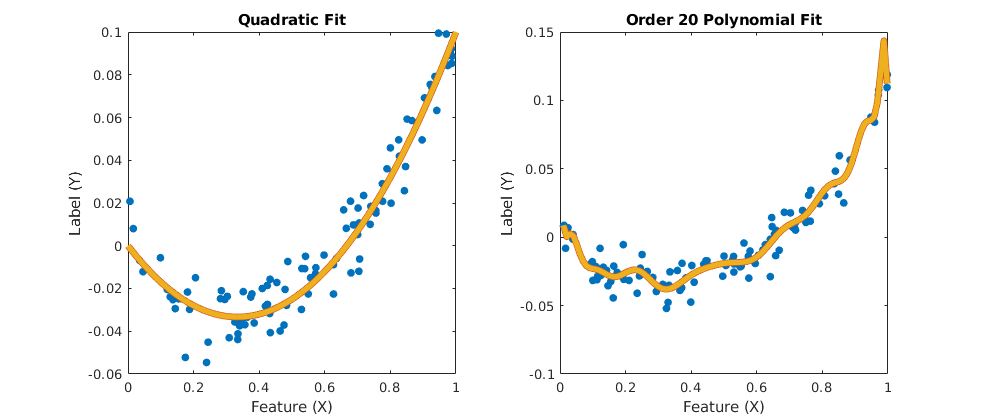
\includegraphics[width=\textwidth]{overfitting.png}
    \caption{The figure on the left is the result of an optimization constrained to second order polynomials while the figure on the right is the result of a $20^{th}$ order constraint.  The second order constraint achieves a result closer to the underlying curve.}
    \label{fig:poly_reg}
\end{figure}

\subsection{Training, Validation, and Testing}
Using the loss function over all data points is not a suitable measure of the success of a machine learning algorithm.  As discussed in section \ref{sec:overfitting}, models which fit the underlying function worse may easily achieve a better overall loss.  In fact for any finite data set that could feasible represent a function, it is easy to find a function in the form of a hash table that can exactly represent the mapping of inputs to outputs.  Of course, this hash table would not ``generalize'' to other data points and wouldn't represent the underlying function in a meaningful way.  

To help obtain a true measure of success, it is standard to separate the data into three parts: training, validation, and testing.  Essentially, training is used to tune regular parameters, validation is used to tune hyperparameters (e.g. with grid search), and testing is used only to evaluate the effectiveness of the algorithm.  If a model function is guilty of overfitting, it will be revealed by a low training loss and a high testing loss.  Measuring the validation loss over time can also be used for a simple form of regularization called \textit{early stopping}.  In early stopping, training is stopped when the validation loss begins to increase.  Of course validation loss may be noisy so usually the loss over time is smoothed and a human hand picks the time to stop.

%\section{Natural Language Processing}
%\subsection{Tokenization}

%\section{Neural Networks}
%A neural network is a class of mathematical function which uses non-linearities in order to increase representational power as compared to simple linear models.  They differ from other non-linear models like logistic regression by having multiple ``layers'' of nonlinearity between the input and the output.  These non-linearities are called \textit{activation functions}.  The multilayer perceptron is a simple example of neural network which is covered in the following section.

\subsection{Multilayer Perceptron}
A multilayer perceptron is a function $f:\mathbb{R}^n\rightarrow \mathbb{R}^m$. Given some vector $x\in \mathbb{R}^n$ of inputs, the output vector $f(x)\in\mathbb{R}^m$ of a multilayer perceptron is given by equation \ref{eq:mlp}
\begin{align}\label{eq:mlp}
    f(x) = \vec{\sigma_p} \circ T_p \circ\cdots\circ \vec{\sigma_2}\circ T_2\circ \vec{\sigma_1} \circ T_1\circ x
\end{align}
The functions $T_1,\dots,T_p$ are assumed to be affine and often represented as matrix multiplications plus constants.  The functions $\vec{\sigma_1},\dots,\vec{\sigma_p}$ are assumed to be nonlinear, each of these is an activation function.  In order for equation \ref{eq:mlp} to make sense, one must assume that the dimensions of each function are compatible with one another.  Activation functions are usually simple functions which operate on an element-by-element basis.  Here the neural network described by \ref{eq:mlp} has $p+1$ layers.  Each activation function adds a layer to the \textit{input layer} which consists of $x$ alone.  Note that the final activation function $\vec{\sigma}_p$ is optional.  It will usually be included if the neural network is performing a classification task and excluded if performing a regression task.

In reference to the previous section, the loss function, $L$ for a neural network classifier is typically given by cross entropy:
\begin{align}
    l(f,x,y) &= \frac{1}{m}\sum_{i=1}^m y_i\log(f_i(x)) + (1-y_i)\log(1-f_i(x))\\
    L(f,X,Y) &= \frac{1}{N}\sum_{i=1}^N l(f,X_i,Y_i)
\end{align}
 and $\vec{\sigma_p}$ is typically given by the softmax function:
\begin{align}
    \vec{\sigma}(\vec{x}) = \frac{e^{x_i}}{\sum_{i=1}^N e^{x_i}}
\end{align}
\subsection{Universal Approximation Theorem}
The simplest multilayer perceptron has three layers: the input, hidden, and output layers.  In this case, the network function is simply given by
\begin{align}
f(x) = T_2 \circ \vec{\sigma} \circ T_1 \circ x
\end{align}
Part of what makes neural networks of the above form so attractive is that they are simple yet powerful.  Given fairly weak constraints on the activation functions, it is possible to represent any univariate continuous function on a compact set arbitrarily well with some $T_1,T_2$ with finite dimensional codomains. \cite{gc89} This has been proven for the $L^1$ norm, $L^2$ norm, and the $L^\infty$ norm.  To be specific, a univariate \textit{sigmoidal} function is defined as $\sigma: \mathbb{R}\rightarrow \mathbb{R}$ and any function satisfying
\begin{align}
\sigma(t) \rightarrow
\begin{cases}
1 \text{ as } t\rightarrow \infty\\
0 \text{ as } t\rightarrow -\infty
\end{cases}
\end{align}
Define $\vec{\sigma}$ as the vectorization of $\sigma$.  That is, 
\begin{align}
\vec{\sigma}(x)_i = \sigma(x_i)
\end{align}
Two common choices for such a function in neural networks are the logistic function (given by $\sigma(x) = \frac{1}{1-e^x})$ and the $\tanh$ function (given by $\tanh(x) = \frac{e^x - e^{-x}}{e^x + e^{-x}}$).  The universal approximation theorem says that given a compact set, $I\subset \mathbb{R}^m$, $\epsilon > 0$, and this sigmoidal activation, one can pick $T_1,T_2$ such that any of the conditions in equations \ref{eq:linf}-\ref{eq:l2} could be met.
\begin{align}
\label{eq:linf}||f(x) - g(x)||_\infty &< \epsilon \text{ } \forall x\in I \\
\label{eq:l1}||f(x) - g(x)||_1 &< \epsilon \text{ } \forall x\in I\\
\label{eq:l2}||f(x) - g(x)||_2 &< \epsilon \text{ } \forall x\in I
\end{align}
for any function, $g(x)$ in $C(I)$, $L^1(I)$, or $L^2(I)$ respectively.

However, as the author of \cite{gc89} writes, this theorem gives no upper bound on the dimensionality of the output of $T_1$ and posits that this value is likely very large.  In addition, one is still left the task of determining the functions $T_1$ and $T_2$ which produce the desired results.  Since they are affine and $x$ is finite dimensional, they may be represented with matrices and so the task is to find the corresponding coefficients, i.e. training.  This is usually done with a very approximate algorithm, stochastic gradient descent, covered in section \ref{sec:sgd}.  

The two main issues of training is that the algorithms are not exact, and the size of matrices required to represent the function may be too large to be computationally feasible. For these reasons, most neural network research is devoted to creating structures which facilitate learning or reduce the computational complexity of a model.  Section \ref{sec:training} discusses several training strategies which help learn the correct parameters as well as avoid the problem of overfitting.  Section \ref{sec:rnn} describes recurrent neural networks, a structure which is particularly efficient at learning features of time series.  

\section{Training Algorithms}\label{sec:training}
Neural networks are highly nonlinear, non-convex functions and therefore very difficult to train efficiently.  Colloquially, one can think of any kind of machine learning training as being in a large field and trying to find the lowest valley or the highest peak.  Unfortunately, one cannot see the terrain nearby and only have local information about the current point.  Stochastic gradient descent is the ubiquitous choice for almost every training scenario.  Powerful extensions of stochastic gradient descent have also been invented, such as the Adam optimizer.

\subsection{Newton's Method}
If weights are allowed to range over an open set (in fact they are usually over $\mathbb{R}$) then $\nabla L = 0$ is a necessary condition for the loss to be minimum.  This condition also guarantees the function is at least at a global minimum or maximum.  This equation is usually not directly solvable for nonlinear functions like neural networks.  However, Newton's method can be used to successively approximate it.  In reference to the loss function discussed in section \ref{sec:machine_learning}, let $L(g,x,y) = L(w)$ where $w$ is the vector of weights for the neural network.  Applying Taylor's Formula to the gradient:
\begin{align}
\nabla L(w+\Delta) &\approx \nabla L(w) + HL(w)\Delta
\end{align}
where $H$ is the Hessian matrix of $L$. 
To find the zero of $\nabla L$, set $L(w+\Delta) = 0$ resulting in  
\begin{align}\label{eq:newton}
\Delta &= -[HL(w)]^{-1}\nabla L(w)
\end{align}
Which finally yields the update step
\begin{align}\label{eq:newtons}
w \gets w - [HL(w)]^{-1}\nabla L(w)
\end{align}

The issue with this method is in the computation of the Hessian and its inverse.  Most modestly complex neural networks have at least thousands of parameters meaning that $H$ will be a very large matrix (containing the number of parameters squared).  Not only does this put a strain on memory resources, but the inversion of such a matrix is extremely time consuming.  In addition, the loss is defined over every point in the data set meaning even computing the loss is very time consuming for large data sets, let alone its derivative with respect to all parameters.  SGD mitigates these issues by avoiding the computation of both the loss or the Hessian.

\subsection{Stochastic Gradient Descent}\label{sec:sgd}
Stochastic gradient descent (SGD) is a very simple algorithm which pushes the parameters of a model in the direction associated with the steepest loss decrease.  First, assume that the loss function $L(g,x,y)$ discussed in section \ref{sec:machine_learning} can be broken down as a sum of loss functions over each feature-label pair, that is:
\begin{align}
L(g,x,y) = \sum_{i=1}^N l(g,x_i,y_i)
\end{align}
Given an initial set of weights (often initialized pseudo-randomly), SGD follows the update in equation \ref{eq:sgd}.
\begin{align}\label{eq:sgd}
w \leftarrow w - \eta\nabla l(g,x_i,y_i)
\end{align}
where $\eta$ is a real valued hyperparameter called the learning rate.

Equation \ref{eq:sgd} says that SGD alters the weights in the direction of the negative gradient.  Because the the gradient of a function normally points in the direction of maximum increase, this update points in the direction of maximum decrease.  This type of learning strategy is called \textit{hill climbing}.  Note that the updates applied to the weights are entirely based on a local calculation, the gradient.  The algorithm is stochastic in the sense that the updates depend only on the \textit{randomly chosen} $x_i,y_i$ pair.  Using the function $l$ instead of $L$ is akin to stochastically approximating the true gradient of $L$ with one of its components.  

Supposing the algorithm halts since all gradients of $l(g,x_i,y_i)$ are zero, this would imply that the gradient of $L$ is given by
\begin{align}
\nabla L(g,x,y) = \nabla \sum l(g,x_i,y_i) = \sum \nabla l(g,x_i,y_i) = 0
\end{align}
 which is a necessary, but not sufficient condition for having a global minimum at that point.  In practice this never occurs and the algorithm is said to converge if the changes become ``small enough.''  It is obvious that for complicated functions like neural networks, this method in general does not produce optimum results.  That is, the coefficients to which this algorithms converges do not minimize the loss function, $L$.  However as mentioned with regard to overfitting, completely minimizing the loss function does not necessarily yield good results anyway.  One may force convergence of the algorithm by applying an exponential decay to the learning rate.  This method is known as exponential learning decay.  Note that this may not actually force convergence in scenarios where the gradient grows exponentially or faster.  

SGD is an approximation of Newton's method in two senses.  At each step, value $[HL(w)]^{-1}$ is approximated by $\eta I$ and $L(g,x,y)$ is approximated as $l(g,x_i,y_i)$.  One obvious issue with using SGD is that one must choose the learning rate with little or no guidance from the data.  Usually good values between $10^{-3}$ and $1$ work fairly well as initial learning rates.  This arbitrary factor has caused others to develop more sophisticated techniques which essentially estimates the best learning rate at a given point in time during training.

\subsection{Adam Optimizer}
The Adam Optimizer algorithm \cite{pd14} essentially calculates how ``reliable'' each element of the gradient vector is and weights the updates accordingly.  It accomplishes this by estimating the first and second moments of the gradient vector with a moving average exponential filter, essentially estimating the mean and variance of each element.  The update weights are inversely proportional to the square root of the second moment, as described in algorithm \ref{alg:adam}.

\begin{algorithm}
\begin{algorithmic}[1]
\begin{spacing}{1.0}
    \caption{\textit{Adam Optimizer}.  $(A\circ B)_{ij} = A_{ij}\times B_{ij}$ is the Hadamard product of $A$ and $B$.  $(A \oslash B)_{ij} = A_{ij}/B_{ij}$ is Hadamard division.  The hyperparameter $\alpha$ is similar to the learning rate, $\eta$ in SGD.  $\beta_1$ and $\beta_2$ are filter coefficients representing smoothing amount.  The value $\epsilon$ is an arbitrary small number to avoid division by $0$.}
    \Require $\beta_1,\beta_2$
    \Require $\alpha$
    \Require $w$
    \Require $l(w,x,y)$
    \State{$m \gets \vec{0}$}
    \State{$v \gets \vec{0}$}
    \State{$t \gets 0$}
    \While{$w$ not converged}
        \State{$t\gets t + 1$}
        \State{$G \gets \nabla l(w,x_{t\bmod N},y_{t\bmod N})$}
        \State{$m \gets \beta_1 m + (1-\beta_1)G$}
        \State{$v \gets \beta_2 v + (1-\beta_2)(G\circ G)$}
        \State{$\hat{m} \gets m/(1-\beta_1^t)$}
        \State{$\hat{v} \gets m/(1-\beta_2^t)$}
        \State{$w\gets w - \alpha \times \hat{m}\oslash (\sqrt{\hat{v}+\epsilon})$}
    \EndWhile
\label{alg:adam}
\end{spacing}
\end{algorithmic}
\end{algorithm}

Adam requires several more hyperparameters as compared to SGD, but the results tend to be less dependent on them.  The parameters $\beta_1$ and $\beta_2$ represent filter coefficients for estimating the first and second moments of the gradient.  Figure \ref{fig:freqz} shows the frequency response with beta ranging from 0.8 to 1.0 logarithmically. Observe that lower $\beta$ represents a bias for lower frequencies.  It turns out that these estimates of $m$ and $v$ are biased, but can be fixed with a simple multiplicative correction (lines 9 and 10).  If you consider the second moment to represent the noise power present in the signal, then the quantity $\hat{m}\oslash \hat{v}$ somewhat represents the signal to noise ratio.  Using this interpretation, this update weighting is somewhat similar to a Wiener filter where the components of the signal which have the most noise are proportionally suppressed.

\begin{figure}
    \centering
    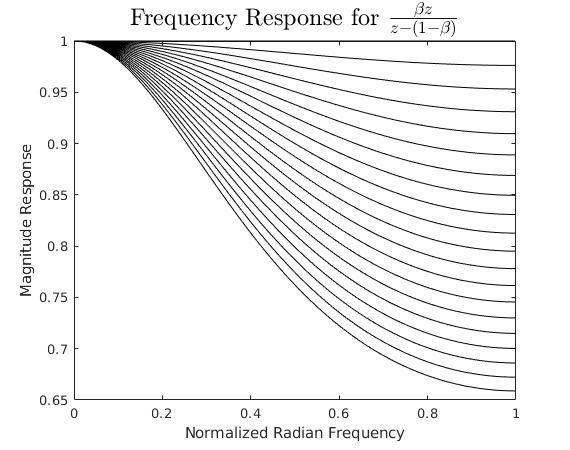
\includegraphics[width=0.8\textwidth]{freqz.png}
    \caption{Frequency response for several moving average exponential filters.  Lower lines are associated with lower values of $\beta$.}
    \label{fig:freqz}
\end{figure}

\subsection{Automatic Differentiation}\label{sec:autodiff}
In all of the previous training algorithms, computation of the gradient of the loss, $\nabla l(w,x,y)$ has been ignored.  This section briefly discuss automatic differentiation, a powerful dynamic programming algorithm for computing the gradient of an arbitrary differentiable function.

Consider some function which depends on multiple variables.  In computing the function, it will likely be expressed as the compositions of other functions.  An example function taken from \cite{ab15} is given below.
\begin{align}\label{eq:autodiff}
f(x_1,x_2) = \log(x_1) + x_1\times x_2 - \sin(x_2)
\end{align}
Equation \ref{eq:autodiff} is a composition of $\log$, $\times$, $\sin$, $+$, and $-$.  This composition can be captured in the form of a graph, as seen in figure \ref{fig:graph}.  Starting at the output and working backwards, one can compute the output of the previous required computation.  Automatic differentiation works in much the same way that a normal computation is performed except by applying the chain rule.  For example, in order to compute the derivative with respect to $x_1$ at node $v_7$, representing the function $[\log(x_1) + x_1\times x_2] - [\sin(x_1)]$, compute $D_{x_1}[\log(x_1) + x_1\times x_2] - D_{x_1}[\sin(x_1)]$.  In order to find the two component values, look at the nodes associated with those functions where the derivative will either already be computed, or where one will compute the derivative by climbing up the graph the same as in the previous step.  Applying this algorithm for all inputs yields the gradient.

\begin{figure}
    \centering
    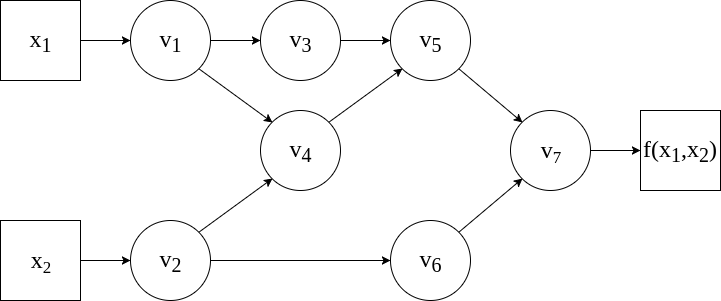
\includegraphics[width=0.8\textwidth]{graph.png}
    \caption{Graph reproduced from \cite{ab15}.  Each node represents a function of the incoming nodes.}
    \label{fig:graph}
\end{figure}

\section{Recurrent Neural Networks}\label{sec:rnn}
Recurrent neural networks are a subset of neural networks which have a key distinction from multilayer perceptrons: they can be applied to data of arbitrary length.  To give more detail we introduce some notation.  Let the set of all n-dimensional vector sequences (finite or otherwise) be given by
\begin{align}
S_n = \{s:Z \rightarrow \mathbb{R}^n; \text{ } \forall Z\subseteq\mathbb{Z}^+\}
\end{align}
While a multilayer perceptron is a function $f:\mathbb{R}^n\rightarrow \mathbb{R}^m$, a recurrent neural network is a function $R: S_n \rightarrow S_m$.

\subsection{Overview}

Of course, the multilayer perceptron could be extended match this if one windows the sequence, compute the output, and then slide the input window.  What truly separates RNNs from MLPs is the fact that an RNN's output depends on its ``state'' at previous time steps.  In particular, denoting the input sequence as $x = (x_1,x_2,\dots,x_k)$ then the states at time steps $1,\dots,k$ are given by equations \ref{eq:rnn_st_start}-\ref{eq:rnn_st_end}.

\begin{align}\label{eq:rnn_st_start}
S_1 &= s(x_1,S_0)\\
S_2 &= s(x_2,s(x_1,S_0))\\
S_3 &= s(x_3,s(x_2,s(x_1,S_0)))\\ \nonumber
&\vdots\\
S_k &= r(x_k,S_{k-1})\label{eq:rnn_st_end}
\end{align}
And the outputs are given by equations \ref{eq:rnn_out_start}-\ref{eq:rnn_out_end}
\begin{align}\label{eq:rnn_out_start}
R_1 &= r(x_1,S_1)\\
R_2 &= r(x_2,r(x_1,S_1))\\
R_3 &= r(x_3,r(x_2,r(x_1,S_1)))\\ \nonumber
&\vdots\\
R_k &= r(x_k,S_{k})\label{eq:rnn_out_end}
\end{align}
If the output sequence is finite, the output of the RNN is the sequence $R(x) = (R_1,R_2,\dots,R_k)$, else it is given by $R(x) = (R_1,R_2,R_3,\dots)$.  The function $s:\R^n \times \R^p \rightarrow \R^p$ is called the state transition function, and the function $r:\R^n \times \R^p \rightarrow \R^p$ is called the output function.  It is assumed that $S_0$ is some arbitrary fixed value (usually zero), called the initial state.  Note that this framework is all very similar to the state-space model, ubiquitous in control theory, except that nonlinearity is allowed in this case.

We can see that the adapted version of the MLP would not be able to represent functions which depend on inputs from time steps farther apart than the length of the window.  In this regard, MLPs are to RNNs as FIR filters are to IIR filters.  Unfortunately because of the non-linearities introduced in RNNs, there is no simple method of analyzing stability, and so training of RNNs has proved difficult throughout their history.  Recent advancements like the long short-term memory unit and dropout have made the training of large RNNs possible.

\subsection{Early Networks}
Some of the first known RNNs, now known as ``simple recurrent networks'' are the Elman \cite{je90} and Jordan \cite{mj86} networks.  The Elman update equations are given by the following equations:
\begin{align}
S_k &= \sigma_S(W_Sx_k+U_SS_{k-1}+b_S\label{eq:elman_s})\\
R_k &= \sigma_R(W_RS_k+b_R)\label{eq:elman_y}
\end{align}
while the Jordan update equations are given by the equations:
\begin{align}
S_k &= \sigma_S(W_Sx_k+U_R R_{k-1}+b_S) \label{eq:newj_s} \\
R_k &= \sigma_R(W_R S_k + b_R) \label{eq:newj_y}
\end{align}
The Elman equations are already in a form consistent with the given framework.  Substituting the second Jordan equation into the first yields the following:
\begin{align}
S_k &= \sigma_S(W_Sx_k+U_R \sigma_R(W_R S_{k-1} + b_R)+b_S)\label{eq:jordan_s}\\
R_k &= \sigma_R(W_R S_k + b_R) \label{eq:jordan_y}
\end{align}
The functions $\sigma_S$ and $\sigma_R$ are sigmoidal activation functions.  The parameters $W_S$,$W_R$, and $U_R$ are matrices, $b_S$ and $b_R$ are bias vectors.

A result analogous to the universal approximation theorem was proved in \cite{hs91}.  Given mild conditions on $r$ and $s$, similar to those of the universal approximation theorem, a recurrent neural net of sufficiently large size is capable of simulating a universal Turing machine.  This means that even a simple RNN (like a Jordan or Elman network) could compute any function, or perform any algorithm that can be performed by a regular computer.  Of course just as with the universal approximation theorem, this says nothing about what is required to train such a network, how many resources it would require, or how efficiently it would operate.

\subsection{Long Short-Term Memory}
Consider computing the derivative of the output of a recurrent neural network with respect to one of its feedback weights, $w$.  By the chain rule:
\begin{align}\label{eq:rnn_deriv}
\frac{d}{dw}R_k(w,x_k,S_k) &= r'(w,x_k,S_k)\times s'(w,x_{k-1},S_{k-1})\times \nonumber
\\&s_{k-1}'(w,x_{k-2},S_{k-2})\times \dots
\times s'(w,x_2,S_1)\times s'(w,x_1,S_0)\\
&= R_k'(x_k,S_k)\prod_{i=1}^k s'(x_i,S_{i-1})
\end{align}
The log derivative is given by
\begin{align}
log(R_k'(x_k,S_k)) + \sum_{i=1}^k \log(s'(x_i,S_{i-1}))
\end{align}
Although it is hard to formally say anything about this value, intuitively since values are being accumulated over time, the log derivative acts as an unstable system.  If the value goes to some very negative number, then the derivative will become extremely small.  On the other hand if the value goes to some very large number, the derivative will become extremely large.  These issues are known as the problems of vanishing and exploding gradients respectively.

The driving cause for exploding or vanishing gradient is that when the state transitions from one time step to another, it is multiplied by some matrix.  The chain rule causes this matrix to be multiplied by itself repeatedly in the derivative calculation which results in either exponential blow up or decay.  The only way to maintain a relatively constant value is for that matrix to be identity, which is exactly the idea behind the long short-term memory (LSTM) unit. \cite{sh97} The update equations for the original LSTM RNN are given by the following:
\begin{align}\label{eq:lstm_start}
i_k &= \sigma_i(W_ix_k + U_iR_{k-1} + b_i)\\
o_k &= \sigma_o(W_ox_k + U_oR_{k-1} + b_o)\\
c_k &= \sigma_c(W_cx_k + U_cR_{k-1} + b_c)\\
S_k &= S_{k-1} + i_k \circ c_k\\
R_k &= \sigma_R(S_k) \circ o_k\label{eq:lstm_end}
\end{align}
Where $\circ$ represents Hadamard (entry-wise) multiplication.

It is easy to see that these equations satisfy the update equations of a standard RNN, as defined.  The direct ``connection'' between $S_k$ and $S_{k-1}$ helps mitigate the issue of vanishing or exploding gradient.  It is important that $i_k$ and $c_k$ can have different signs so that the state is not stuck accumulating in one direction.  For this reason, $\sigma_i$ is usually $\tanh$ while $\sigma_o$ is usually the logistic function.

The model was later extended by \cite{fg00} with what they called a forget gate.  The forget gate, described by the new update equations \ref{eq:forget_1}-\ref{eq:forget_2}, allows the network to essentially discard information in the state and start again.
\begin{align}
f_k &= \sigma_f(W_fx_k + U_fR_{k-1} + b_f)\label{eq:forget_1}\\
S_k &= S_{k-1}\circ f_k + i_k \circ c_k\label{eq:forget_2}
\end{align}

The same group responsible for the invention of forget gates also invented the peephole LSTM. \cite{fg00_2} In this modification of the forget gated LSTM, all instances where the output of the neural network is fed back are replaced with the internal state instead.  For example equation \ref{eq:lstm_start} becomes 
\begin{align}\label{eq:peephole}
i_k = \sigma_i(W_ix_k + U_iS_{k-1})
\end{align}
and so on.

\subsection{Training RNN's}\label{sec:rnn_training}
Recurrent neural networks are trained in much the same way that a standard neural network is trained with one key complication, the input is potentially unbounded.  This means that the number of computations is potentially unbounded and so there is no single graph representing the network.  To solve this issue in computing gradients, the neural network is \emph{unfolded} for some finite amount of time steps.  Any input which goes past the maximum time step is discarded in the computation.

Dropout is a regularization method that can be used to avoid overfitting when training neural networks.  It as applicable to a wide range of neural net models, though its application to recurrent neural networks is slightly more complex.  Essentially, dropout randomly zeros out certain values in the neural net at every time step.  Dropout can be applied at the input, output, or internal state of an LSTM cell.  It was found that applying dropout to state variables led to poor performance, while applying dropout to the output of a cell led to increased performance. \cite{wz14} This type of RNN regularization simply means changing equation \ref{eq:lstm_end} to:
\begin{align}
R_k &= D(\sigma_R(S_k) \circ o_k)
\end{align}
where $D$ zeros random elements of the vector according to independently and identically distributed Bernoulli distributions.



%\section{Numerical Representation of Language}
%Many modern machine learning techniques require a numerical representation of data and therefore cannot work with natural language directly.  There are several different representations which have advantages and drawbacks.  We will specifically look at vector space representations which are useful for classifying documents.  This chapter will cover the simple bag-of-words model of documents and the more advanced word2vec model.

\subsection{Bag-of-words}
A bag-of-words model is a very simple numerical representation of a text document.  The model assumes that a given document has already been tokenized.  In bag-of-words, a single document is represented as the multiset of all tokens in the document with no regard toward ordering.  This means that the conversion is, in general, not invertible and so the original document cannot be retrieved from this representation.

Consider the document
\begin{center}
\texttt{"This movie is not terrible, this movie is amazing!"}
\end{center}
One possible bag-of-words representation for this document is
\begin{center}
\texttt{\{this, movie, is, not, terrible, this, movie, is, amazing\}}
\end{center}
Notice that the above object is not a set, but a multiset since it contains one or more elements more than once.  Also not that the following example is equivalent, since it contains the same words with the same frequency.
\begin{center}
\texttt{\{this, movie, is, not, amazing, this, movie, is, terrible\}}
\end{center}

This object is conveniently represented as a hash table mapping tokens directly to their frequency in the document like the example in table \ref{tab:hash}
\begin{table}[h]
\centering
\begin{tabular}{ r l }
 this & 3 \\ 
 movie & 3 \\  
 is & 3 \\ 
 not & 1 \\
 terrible & 1 \\
 amazing & 1 \\
\end{tabular}
\caption{Hash table representation of a multiset}
\label{tab:hash}
\end{table}

In the context of comparing two documents, it is sometimes more useful to represent a document as a vector.  If we want to represent every possible document as a vector of the same length, then the number of elements must be equal to the total number of possible tokens, or the size of the vocabulary.  For example, table \ref{tab:hash} might be represented as 
\begin{singlespace}
\begin{align}
x = 
\begin{bmatrix}
0 & \cdots & 3 & \cdots & 3 & \cdots & 3 & \cdots & 1 & \cdots & 1 & \cdots & 1 & \cdots & 0
\end{bmatrix}^\mathsf{T}
\end{align}
\end{singlespace}
\noindent
with dots representing some amount of zeros.  With this representation, one simple measure of document similarity is given by the \textit{cosine similarity}, $s_\theta(d_1,d_2)$, of two document vectors
\begin{align}
s_\theta(x_1,x_2) = \frac{x_1\cdot x_2}{||x_1||_2 ||x_2||_2}
\end{align}
By the Cauchy–Schwarz inequality, this value has an upper bound of $1$, which is achieved if and only if the two documents contain the same words with the same relative frequency.

The vector representation of documents also gives a hint as to how we might represent individual words numerically.  If $i$ is the index associated with the $i^{th}$ word in a vocabulary, then we may associate that word with the standard basis vector $e_i$.  Where every component of $e_i$ is $0$ except for the $i^{th}$ which is $1$.  Let $e_m$ be the standard basis vector associated with word $m$, then the vector represention for a document multiset, $M$, would be given by
\begin{equation}
x = \sum_{m\in M} v(m)e_m
\end{equation}
where $v$ is the multiplicity of element $m$ in $M$.

In most cases, an actual language processing system will not use the raw frequency, $n_{t,d}$, of a term $t$ and document $d$, but rather some term frequency function, $tf(t,d)$, of the raw frequency and given document which results in what is called a \textit{term weighting}.  Common choices are \cite{cm08}:

\begin{enumerate}
\item $tf(t,d) = \{1 \text{ if $t$ appears in $d$; else } 0\}$
\item $tf(t,d) = n_{t,d} / N$, where N is the length of the document
\item $tf(t,d) = \{1 + \log(n_{t,d}) \text{ if $n_{t,d} > 0$; else } 0\}$
\item $tf(t,d) = \frac{1}{2} + \frac{1}{2} \frac{n_{t,d}}{N}$, where N is largest raw frequency in the document.
\end{enumerate}

The inverse document frequency of a term is given by
\begin{equation}
idf(t,D) = -\log d_t/D
\end{equation}
where $d$ is the number of documents containing the term $t$, and $D$ is the number of documents in total.  One of the most common term weightings is then given by the term frequency-inverse document frequency (tf-idf):
\begin{equation}
tfidf(t,d,D) = tf(n,d) \times idf(t,D)
\end{equation}

The bag-of-words model has the advantage of extreme simplicity, however it does not represent complex documents well since it has no regard for ordering.  In addition, using this representation as a feature for machine learning is problematic since the number of features is equal to the vocabulary size which should be a very large number.  We now look at latent semantic analysis, originally a method for indexing documents, which represents words and documents as vectors.

\subsection{Latent Semantic Analysis}
Latent semantic analysis (LSA) is essentially a dimensionality reduction technique similar to principle component analysis.  At it's core is a truncated singular value decomposition (SVD) which is responsible for finding ``key concepts'' behind words.  A set of word vectors for some vocabulary and set of documents can be found with the following steps:

\begin{enumerate}
\item Populate the term-document matrix, $M$: $M_{i,j} = tf(t_i,d_j)$
\item Using SVD, decompose $M$: $M = U\Sigma V^*$.  $U$ and $V$ are unitary while $\Sigma$ is diagonal.
\item Keep the largest $k$ diagonal values in $\Sigma$, remove the other values' rows and columns and call the resulting matrix $\hat{\Sigma}$.
\item The vector corresponding to the $i^{th}$ word is the transpose of the $i^{th}$ row of $U\hat{\Sigma}$, a vector of $k$ elements.
\end{enumerate}
\noindent
Using this method, words which appear in similar frequency across similar types of documents will have similar vectors, in the sense of cosine similarity.  Sample noise is reduced by the dimensionality reduction achieved by truncating $\Sigma$.

\subsection{Word2vec}
Word2vec is an extremely useful model which learns vector representations of individual words.  Word vectors are learned in an unsupervised fashion, meaning that very large, unlabeled datasets can be leveraged during training.  There are two word2vec models which are complementary:  Continuous Bag-of-Words (CBOW) and Continous Skip-gram (Skip-gram).  Continous Bag-of-Words aims to create vectors which maximize accuracy of classifying a word given its surrounding words.  Skip-gram aims to create vectors which maximize the accuracy of predicting surrounding words given the cener word.

The model used for word prediction is very



%\section{Adversarial Machine Learning}
%\input{Adversarial Machine Learning}

\chapter{Problem Statement}
\section{Adversarial Examples}
Adversarial examples were originally defined in the domain of image classification in the form of a constrained optimization problem.  The following definition is similar to \cite{cs14}.  We take images to be vectors in $\mathbb{R}$, and $S$ is a finite set of classes, so that a classifier $f:\mathbb{R}\rightarrow S$ assigns each image a unique class.

\begin{definition}
An adversarial derivation, $x + r \in \mathbb{R}^m$, of an image, $x \in \mathbb{R}^m$ for a classifier, $f$, is a solution to the following optimization problem:
\end{definition}

\noindent
minimize $||r||_2$ subject to:
\begin{enumerate}
\item $f(x + r) \neq f(x)$
\item $x+r \in [0,1]^m$
\end{enumerate}
We may also denote the adversarial derivation as $x^* = x + r$

\noindent
In words, an adversarial derivation is a sample with the minimum distance to a true sample such that it is classified as something different.  We also require that every element stays in the interval $x_n+r_n \in [0,1]$ because actual pixels must remain in some constant bounded interval.

\begin{definition}
A classifier, $f$, over a set, $D$, is a mapping, $f : D\rightarrow \{1,2,\dots,K\} = C$.
\end{definition}

Clearly, this adversarial derivation definition does not translate well to the problem of natural language classification where the domain is not even numeric.  We give a more general  constrained optimization defintion below, which we will adapt to the problem of creating adversarial derivations for text.

\begin{definition}
A distance function, $d$, over a set $S$ is a mapping, $d:S\times S\rightarrow \mathbb{R}$ such that $\forall x,y,z \in S$:
\begin{enumerate}
\itemsep0em
\item $d(x,y) \geq 0$
\item $d(x,y) = 0 \iff x=y$
\item $d(x,y) \leq d(x,z) + d(z,y)$
\end{enumerate}
\end{definition}

\noindent One important example of a distance metric is the discrete metric, given by

\[
\rho(v,v^*) =
\begin{cases}
0 & \text{if $v = v^*$} \\
1 & \text{if $v \neq v^*$} \\
\end{cases}
\]
\noindent
It is also true that if $S$ is a normed linear space, $d(x,y) = ||x-y||$ is a distance metric over that space.

\begin{definition}
Let $d_D$ be a distance function over $D$, and $d_C$ be a distance function over $C$.  Then the point $x^*$ is an adversarial derivation (AD) of $x\in D$ with tolerance $\epsilon > 0$ given by
\begin{equation*}
\begin{aligned}
& \underset{x^*\in D(f)}{\text{min}}
& & d_D(x,x^*) \\
& \text{subject to}
& & d_C(f(x),f(x^*)) > \epsilon
\end{aligned}
\end{equation*}
\end{definition}

\noindent
Note that image classifier would have the domain $[0,1]^m$ and codomain $ \{1,...K\} $ where $K$ is the number of classes.  So the definition of an adversarial derivation for an image classifier is the same as the general definition if we let $\epsilon = 1$, $d_D(x,x^*) = ||x-x^*||^2$, $d_C(y,y^*) = |y-y^*|$.

As long as the function, $f$, has a non-singleton codomain, the constraint is satisfiable for for small enough $\epsilon$.  In the case that the solution does not exist, $\delta = \inf \{d_D(x,x^*) \text{ s.t. } d_C(f(x),f(x^*)) > \epsilon\}$ exists, in which case we may find $\hat{x}$ that is arbitrarily close to $\delta$.  Satisfiability is true from the fact that for any distance metric, $d(y,y^*) > 0$ for $y \neq y^*$.  That all being said, the distance between the sample and the derived sample may be so large that they are easily recognized to be different.  We therefore define a similar problem with very different properties

\begin{definition}
An absolutely adversarial derivation (AAD) of $x$ with similarity $\delta$, difference $\epsilon$, domain metric $d_D$, and codomain metric $d_C$ is given by any solution to the following two constraints.

\begin{equation*}
\begin{aligned}
& & d_D(x,x^*) < \delta\\
& & d_C(f(x),f(x^*)) > \epsilon
\end{aligned}
\end{equation*}
\end{definition}

In this less relaxed version of the problem, a solution may not exist.  In fact, for a given continuous function, $f$, defined on an open domain, and tolerance, $\epsilon$ it is guaranteed that $$\exists \delta > 0 \text{ s.t. } d_C(f(x),f^*(x)) < \epsilon$$ meaning no solution exists.  However, it appeals to a more intuitive concept and allows for the possibility of a model immune to adversarial attacks.  It says that the sample and its absolute adversarial derivation must be sufficiently close and the distance between the model outputs must be sufficiently far.  

It is easy to see that if an AAD exists for a given sample, then any AD is also an AAD.  This means we may solve the more relaxed problem to obtain a valid solution, and so we will work with the more practical objective of creating ADs.

\section{Word Embeddings}
Consider the common scenario of a text classifier which maps plain text files to one of several classes.  It is common for the plain text to first be processed into a sequence of tokens, which are then each assigned an integer resulting in a sequence of integers.

\begin{definition}
Let $s$ be a sequence of characters.  Let $a_n \in \{0,1,\dots,V\} \forall n \in \{0,1,\dots,N\}$ and $E:s\rightarrow \{a_n\}_{n=1}^{N_s}$.  Then we call $E$ an encoder, $V$ the encoder vocabulary size, and $N_s$ the sample length with respect to $E$.
\end{definition}

In plain words, an encoder maps a string to a sequence of bounded integers.  The sequence is some length which depends on both the encoder and the string.  We assume a fixed encoder, and therefore vocabulary size, $V$.  Since, after encoding, the distance between one word and another is arbitrary, we further translate into a one-hot encoded vector.  That is, the integer $n$ is mapped to a vector where the $n^{th}$ element is $1$ and all others are $0$.  This ensures that all vectors representing words are unit norm and the distance between any two different words is the same.  We denote the set of one-hot encoded vectors of size $V$ as $1_V$.

This simple method of representing words as vectors results in a very high dimension representation of all words in the vocabulary, and thus even a very simple linear model would be very large and difficult to train.  Using the word2vec model discussed in the previous chapter, the dimension of this representation can be significantly reduced, while also encoding information about statistical semantic similarity about each word.

\begin{definition}
Let $f: 1_V \rightarrow \mathbb{R}^D$.  We call $f$ a word embedding and we call $D$ the size of $f$, or embedding size.
\end{definition}

\noindent
Let $W \in M_{D\times V}(\mathbb{R})$.  Then clearly any word embedding, $f$, of size $D$ may be represented as the matrix multiplication $Wv$ $\forall v \in 1_V$.  The matrix $W$ is called the embedding matrix.  This numerical representation of words is extremely useful since we can now apply more general and modern techniques to solving the problem of classification.


\section{Adversarial Text Derivation}
\noindent
Now that we have a clear idea of both the domain and numerical representation of words, we may define an adversarial derivation of textual data in the context of a classification model, $f$.  As per the definition of an adversarial derivation, we need only to define the model tolerance, $\epsilon$, as well as the domain metric, $d_D$ and codomain metric, $d_C$.  We will consider primarily two definitions.

\begin{definition}
Let $\{v_i\}_{i=1}^N$ be the sequence of vectors obtained from a given word embedding and text sample, then a discrete adversrial derivation is defined has having domain metric, $d_D(v,v^*) = \sum_i^N\rho(v_i,v_i^*)$, codomain metric $d_C(f(v),f(v^*)) = \rho(f(v),f(v^*))$, and tolerance $\epsilon = 1$.
\end{definition}

That is, a discrete adversarial derivation $\{v_i^*\}$ of sample $\{v_i\}$ is the sample which changes the least amount of words possible, while changing the classification.  This definition is simple, though it may not yield very good results if solved.  For example, a positive movie review, ``This movie was good'' could easily be changed to a negative review by changing just one word resulting in ``This movie was bad''.  These two samples would obviously have different sentiments if read by a human.

%Clearly the codomain metric, $d_C$ and difference, $\epsilon$ make sense for any defintion in this context, but the domain metric has room for improvement which brings us to the next definition.

%\begin{definition}
%A semantic adversarial derivation is defined as having angular distance as the domain metric and the same difference and codomain metric as a discrete adversarial derivation.
%\end{definition}

%If we minimize this objective, then we would tend to use semantically similar words in substitution.  However, this does not necessarily solve the problem of actual sentiment inversion.  For instance, in our embedding the semantically closest (measured with the $l^2$ norm) word to ``bad'' is ``good.''  This makes sense since they are semantically very similar and would be used in the same contexts, but may result in obvious semantic flips.  We will therefore look to other metrics in an attempt to find better results.


\section{Stochastic Gradient Analysis}
\noindent
\begin{definition}
Let the gradient of a model output, $f_i$, with respect to an input vector, $x$ be denoted by $g=\nabla f(x)$.  The total gradient is given by 
\begin{equation}
g_t = \sum_{i=1}^D \nabla f(x)_i
\end{equation}
The gradient norm is given by 
\begin{equation}
g_n = \sqrt{\sum_{i=1}^D |\nabla f(x)_i|^2} = ||\nabla f(x)||_2
\end{equation}
\end{definition}

Both of these measures, along with the gradient itself, are shown for our model as well as a small excerpt of one of the text samples in Figure \ref{fig:saliency}.  We see that the three words with the largest total gradients are ``loved'', ``good'', and ``bad'' which are all sentimental.  First, a differentiable function, $f$, can be locally approximated by
\begin{align}
f(w_j) &\approx f(x_i) + (w_j-x_i)^T\nabla f(x_i) \\
     &= f(x_i) + w_j^T\nabla f(x_i) - x_i\nabla f(x_i) \\
     &= f(x_i) + w_j^Tg - x_i^Tg \label{approx}
\end{align}
Here are considering specificially the affect of replacing the $i^{th}$ input word vector, $x_i$ with the $j^{th}$ embedding word vector, $w_j$ while all other input vectors remain constant.

\begin{definition}

With the above defintions of $x_i$, $w_j$, and $\nabla f(x_i)$, let
\begin{align}
X &= 
\begin{bmatrix}
x_1, x_2, \dots, x_N
\end{bmatrix} \in M_{D\times N}(\mathbb{R})\\
W &= 
\begin{bmatrix}
w_1, w_2, \dots, w_V
\end{bmatrix} \in M_{D\times V}(\mathbb{R})\\
G &= 
\begin{bmatrix}
\nabla f(x_1), \nabla f(x_2), \dots, \nabla f(x_N)
\end{bmatrix} \in M_{D\times N}(\mathbb{R})
\end{align}
\noindent
The approximated perturbation, $f(w_j)-f(x_i)$, of replacing the $i^{th}$ input with the $j^{th}$ embedding word vector is given by 
\begin{align}
    D_{i,j} = (G^TW)_{i,j} - (G^TX)_{i,i}
\end{align}
\noindent
$D$ is called the approximate delta matrix.
\end{definition}
\noindent
For a perfectly linear function, $f$, $D_{i,j} = f(w_j) - f(x_i)$.  We found that for small output differences, the approximation worked fairly well in that a lesser approximate delta tended to produce a lesser actual delta, as seen in figure \ref{fig:dvhat}.  However, the approximation failed almost completely for large differences, as illustrated in figure \ref{fig:outliers}.  This is not surprising given that the model is highly non-linear but it confirms that using the gradient alone is not a reliable technique for discovering adversarial derivations.

\begin{figure}
    \centering
    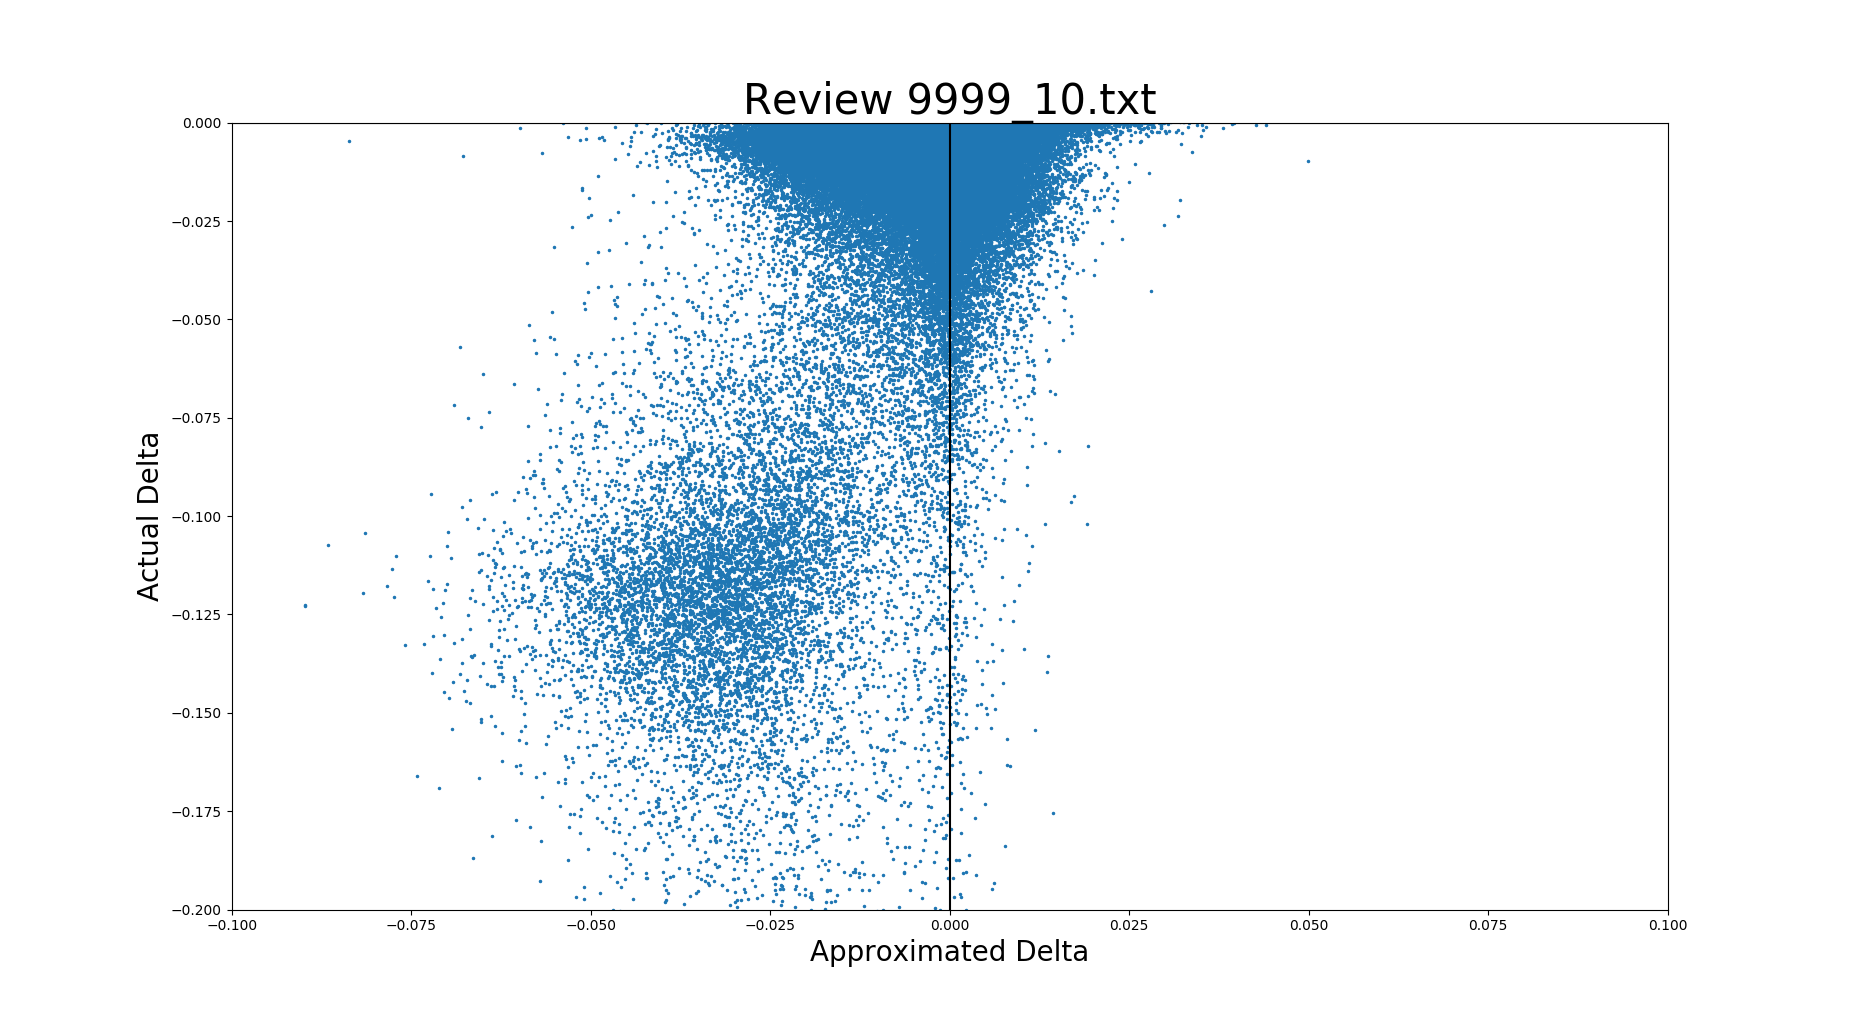
\includegraphics[width=\textwidth]{delta_vs_deltahat.png}
    \caption{Predicted difference in prediction confidence vs. actual difference for sample file 9999\_10.txt}
    \label{fig:dvhat}
\end{figure}

\begin{figure}
\centering
\begin{subfigure}[t]{0.45\textwidth}
  \centering
  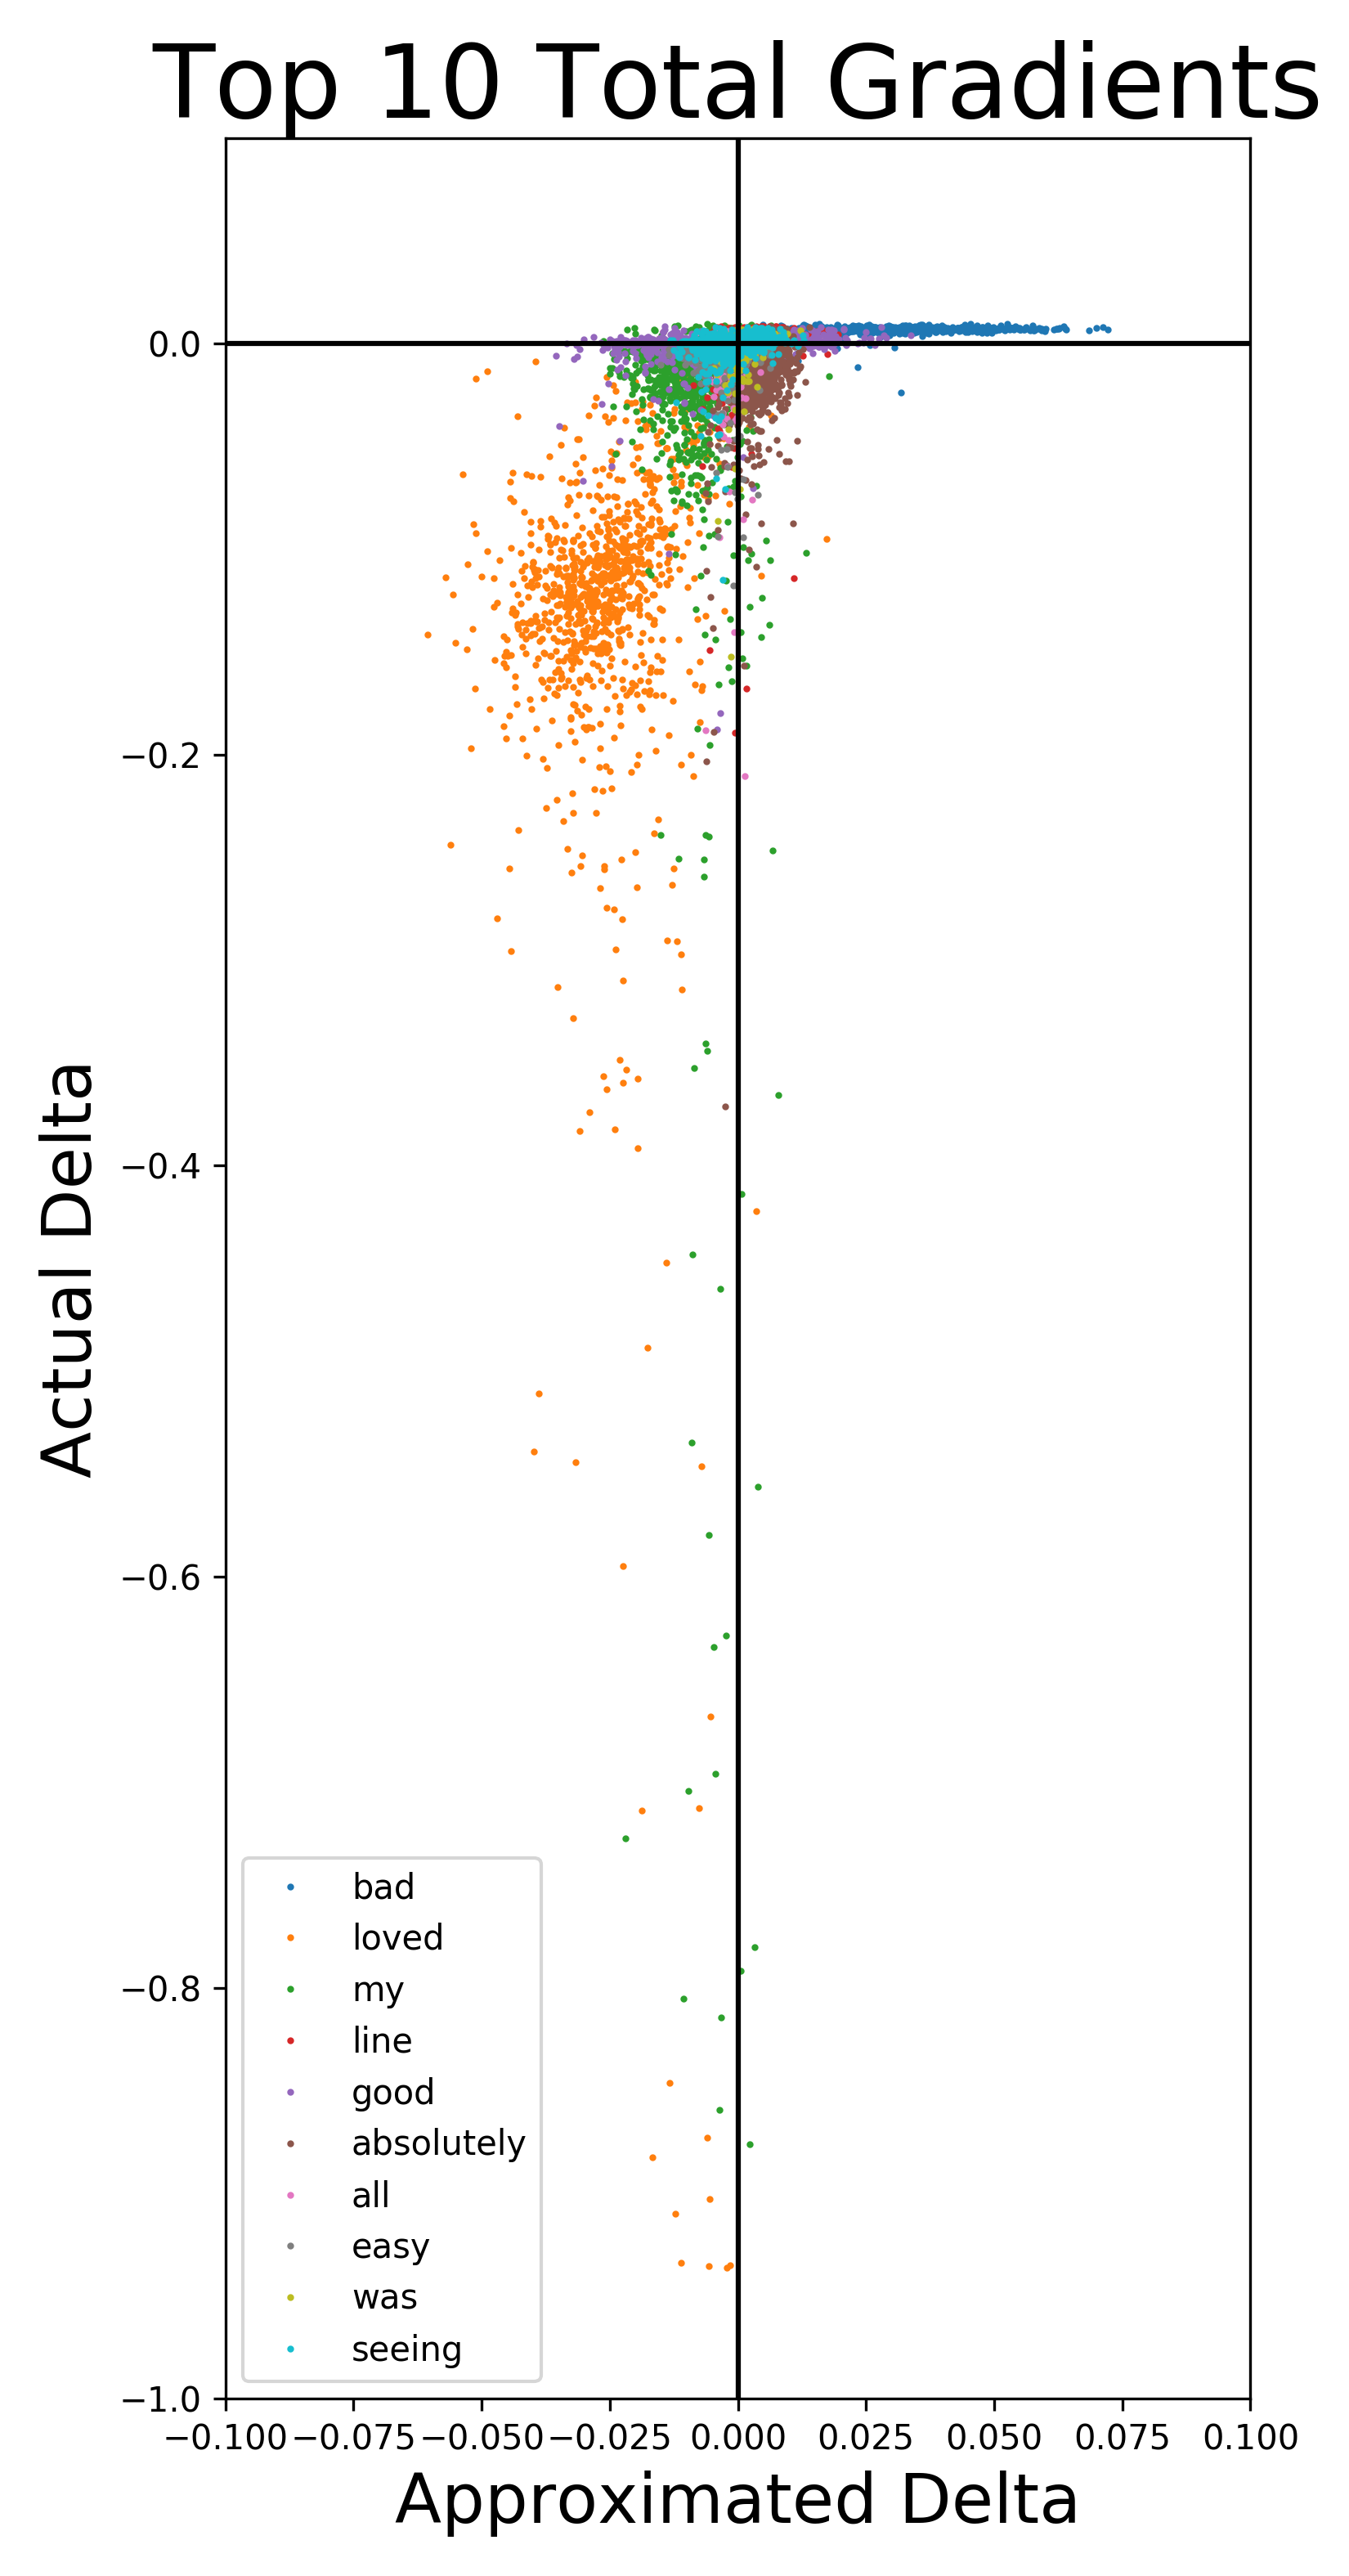
\includegraphics[width=0.9\textwidth]{total_color.png}
  \caption{The words with the top ten largest absolute total gradeints are chosen}
  \label{fig:total_color}
\end{subfigure}\hfill
\begin{subfigure}[t]{0.45\textwidth}
  \centering
  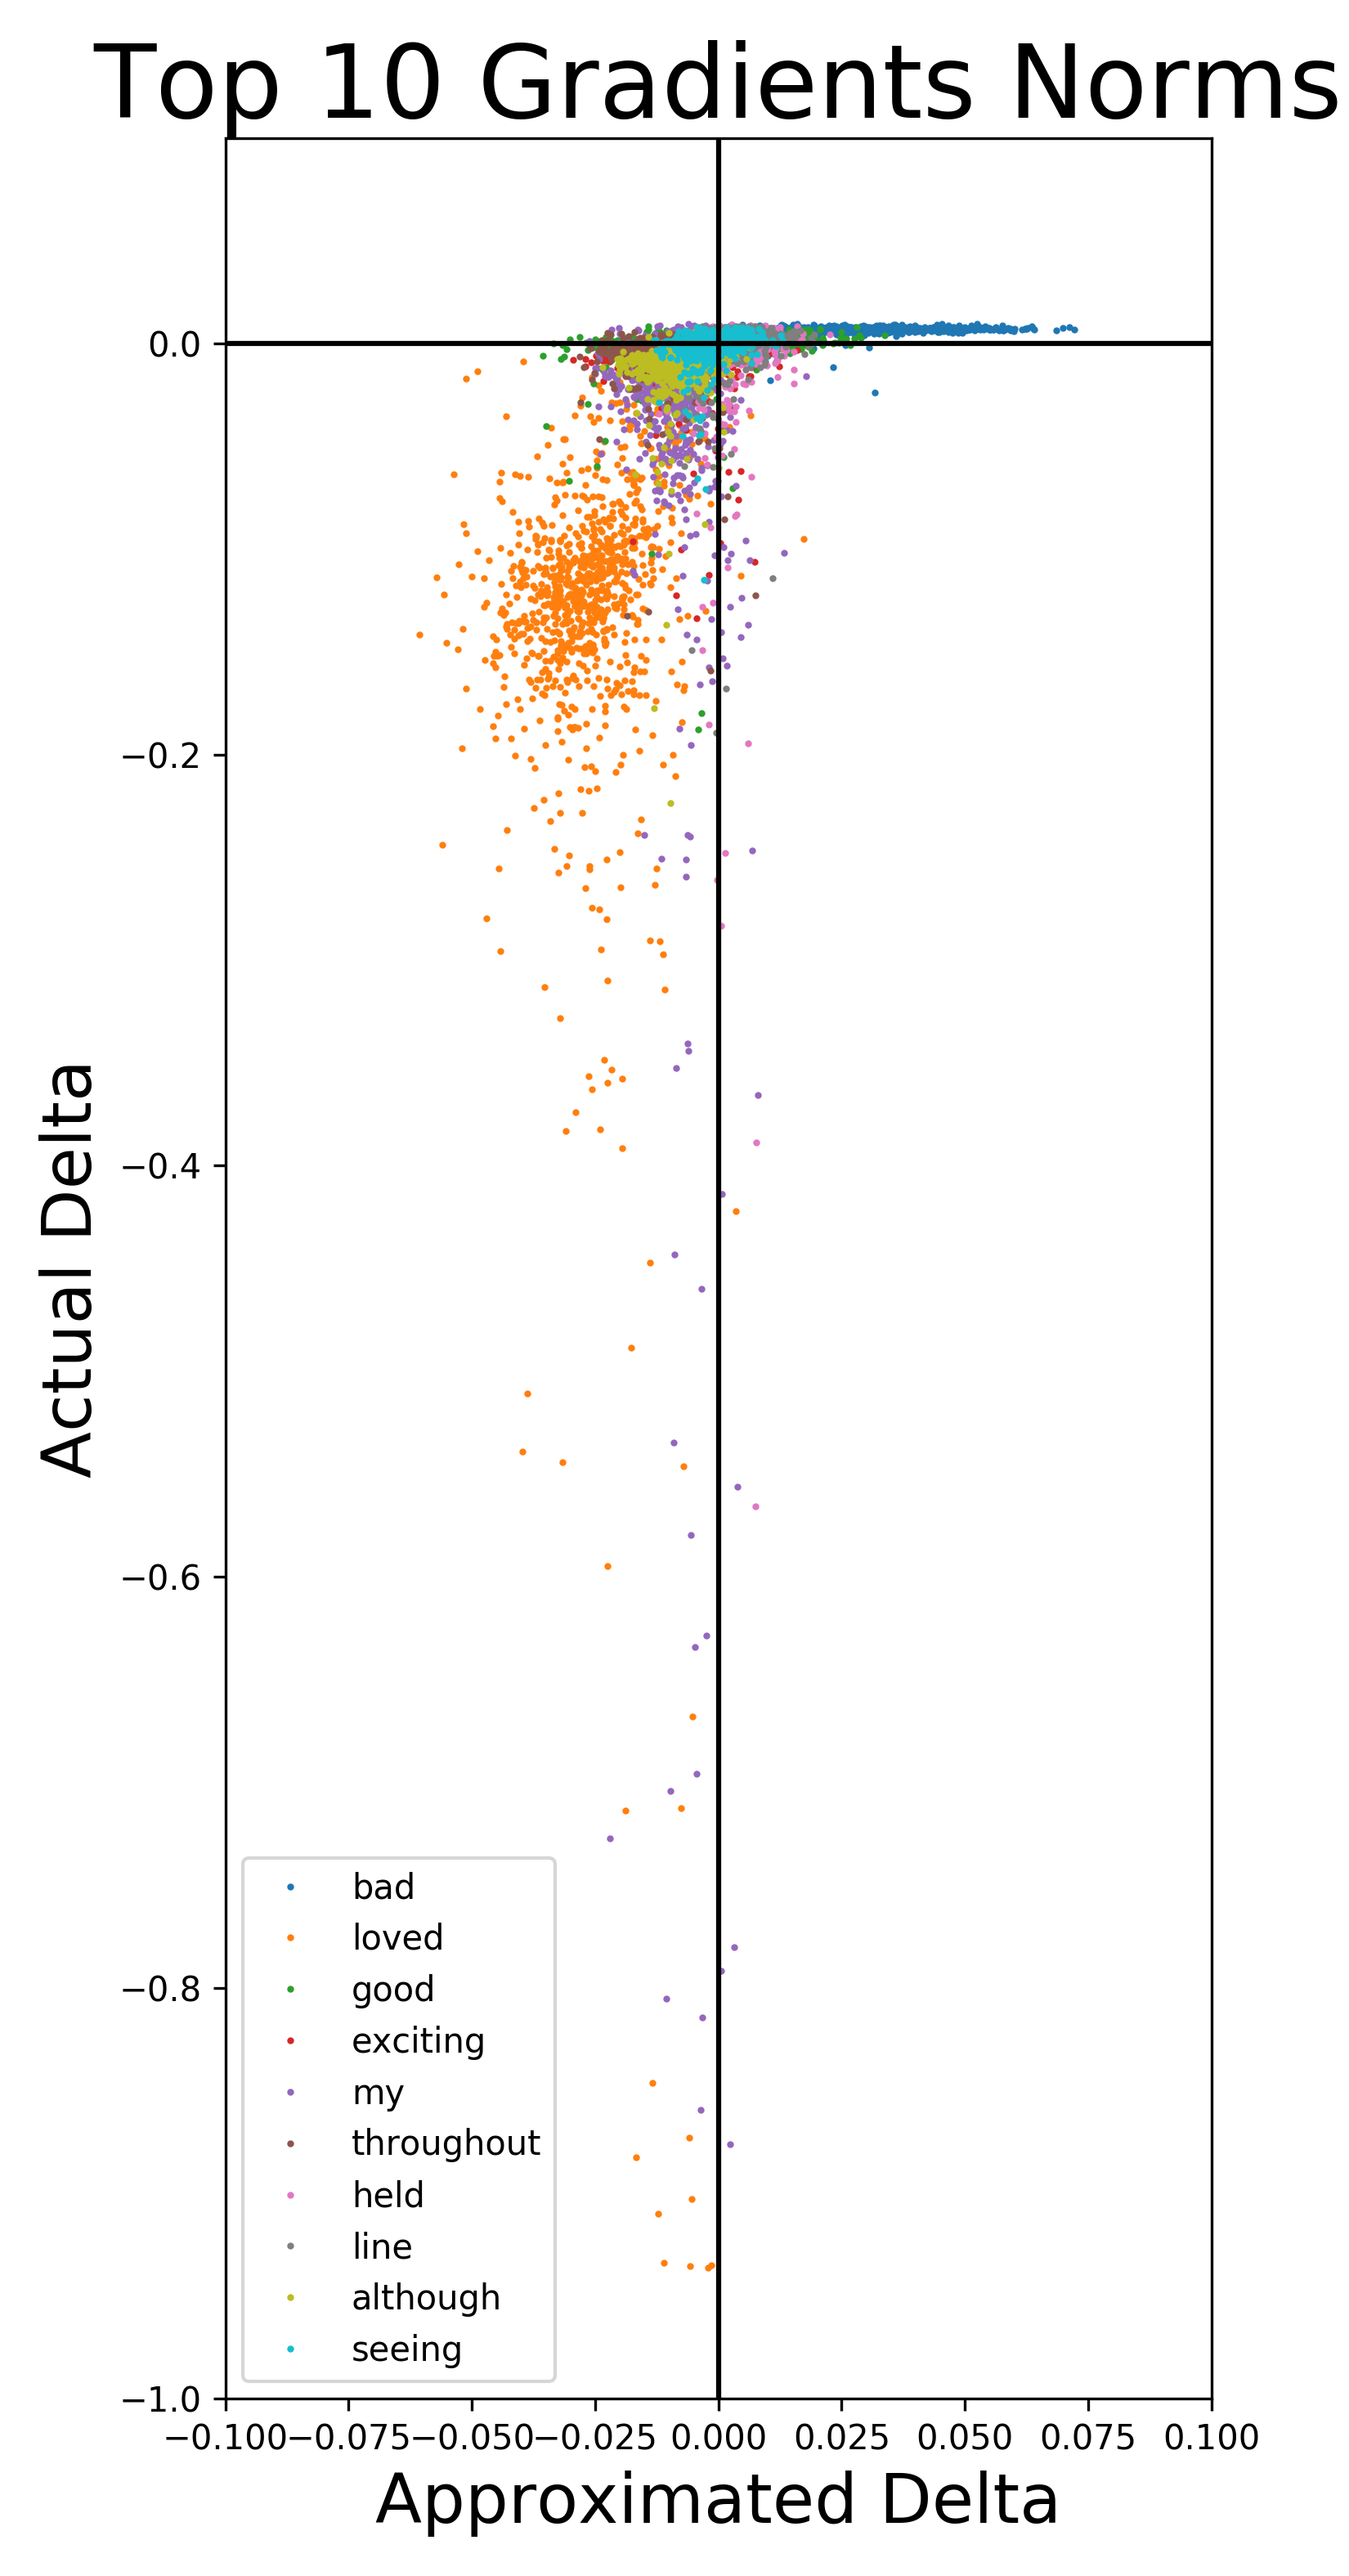
\includegraphics[width=0.9\textwidth]{norm_color.png}
  \caption{The words with the top ten largest gradient norms are chosen}
  \label{fig:norm_color}
\end{subfigure}
\caption{The predicted change in classifier confidence vs. the actual change.  Only the most common 1,000 words are considered in replacement for this example.  The words are listed in the legend in order of decreasing value.}
\label{fig:outliers}
\end{figure}

We see that individual $\hat{D}$ entries are not a good choice for determining which specific words to interchange, but that our measures of gradient may be useful in determining which words are susceptible to attack.  We give motivation with some simplified probabilistic analysis.  Suppose that each of the embedding dimensions is distributed independently and identically across words, with some mean, $\mu$ and variance, $\sigma^2$.  Let $g = \nabla f(x_i)$ for a given word vector, $x_i$ and suppose we replace it with a random word vector, $w_j$.  Recall equation \ref{approx}, we are interested in estimating the term $w_i^Tg = g^Tw_i$ probabilstically since the term $x_i\nabla f(x_i)$ is fixed for a given word.  Let $v=w_i$ and $u=x_i$, then randomly replacing $u$ with another word vector, we have
\begin{equation}
\E{g^Tv} = \E{\sum_{i=1}^D{g_iv_i}} = \sum_{i=1}^D{g_i\E{v_i}} = \mu\sum_{i=1}^D{g_i} = \mu g_t
\end{equation}
\noindent
If we are interested in purposefully altering classification, however, we might be more interested in the expected maximum value of $g^Tv$, that is,
\begin{equation}
Z(g) = \E{\underset{0\leq n\leq V}{\max}\,{g^Tv_n}}
\end{equation}
\noindent
Unfortunately, there is no simple expression which captures this value.  However if we assume that $v_{n,i}$ is distributed normally, we have 
\begin{equation}
Z(g) = \E{\underset{0\leq n\leq V}{\max}\,{g^Tv_n}} = \E{\underset{0\leq n\leq V}{\max}\,{\sum_{i=1}^D{g_i}v_{n,i}}} = \E{\underset{0\leq n\leq V}{\max}\,{p_n}}
\end{equation}
\noindent
where $p_n \sim \mathcal{N}(\mu g_t,\sigma^2 g_n^2)$  There is still no closed form expression for this value, but there is a known \cite{pm07} upper bound:
\begin{align}
Z(g) &\leq \mu g_t + \sigma g_n\sqrt{2\log{V}}\\
\E{\max \hat{D}_{i,*}} &\leq \mu g_t + \sigma g_n\sqrt{2\log{V}} -u^Tg
\end{align}

\noindent
This inequality is intuitively satisfying.  It says that the expected maximum perturbation grows with both the vocabulary size and the norm of the gradient.  The total gradient also plays a role here, increasing or decreasing the expected maximum depending on the sign.  Empirical study of our embedding and classifier show that the term including standard deviation is usually much larger.  It should be noted that the lower bound on the expected minimum, $Y(g)$, is simply given by a sign reversal of the second term:
\begin{align}
Y(g) &\geq \mu g_t - \sigma g_n\sqrt{2\log{V}} \\
\E{\min \hat{D}_{i,*}} &\geq \mu g_t - \sigma g_n\sqrt{2\log{V}} - u^Tg
\end{align}

\begin{figure}
    \centering
    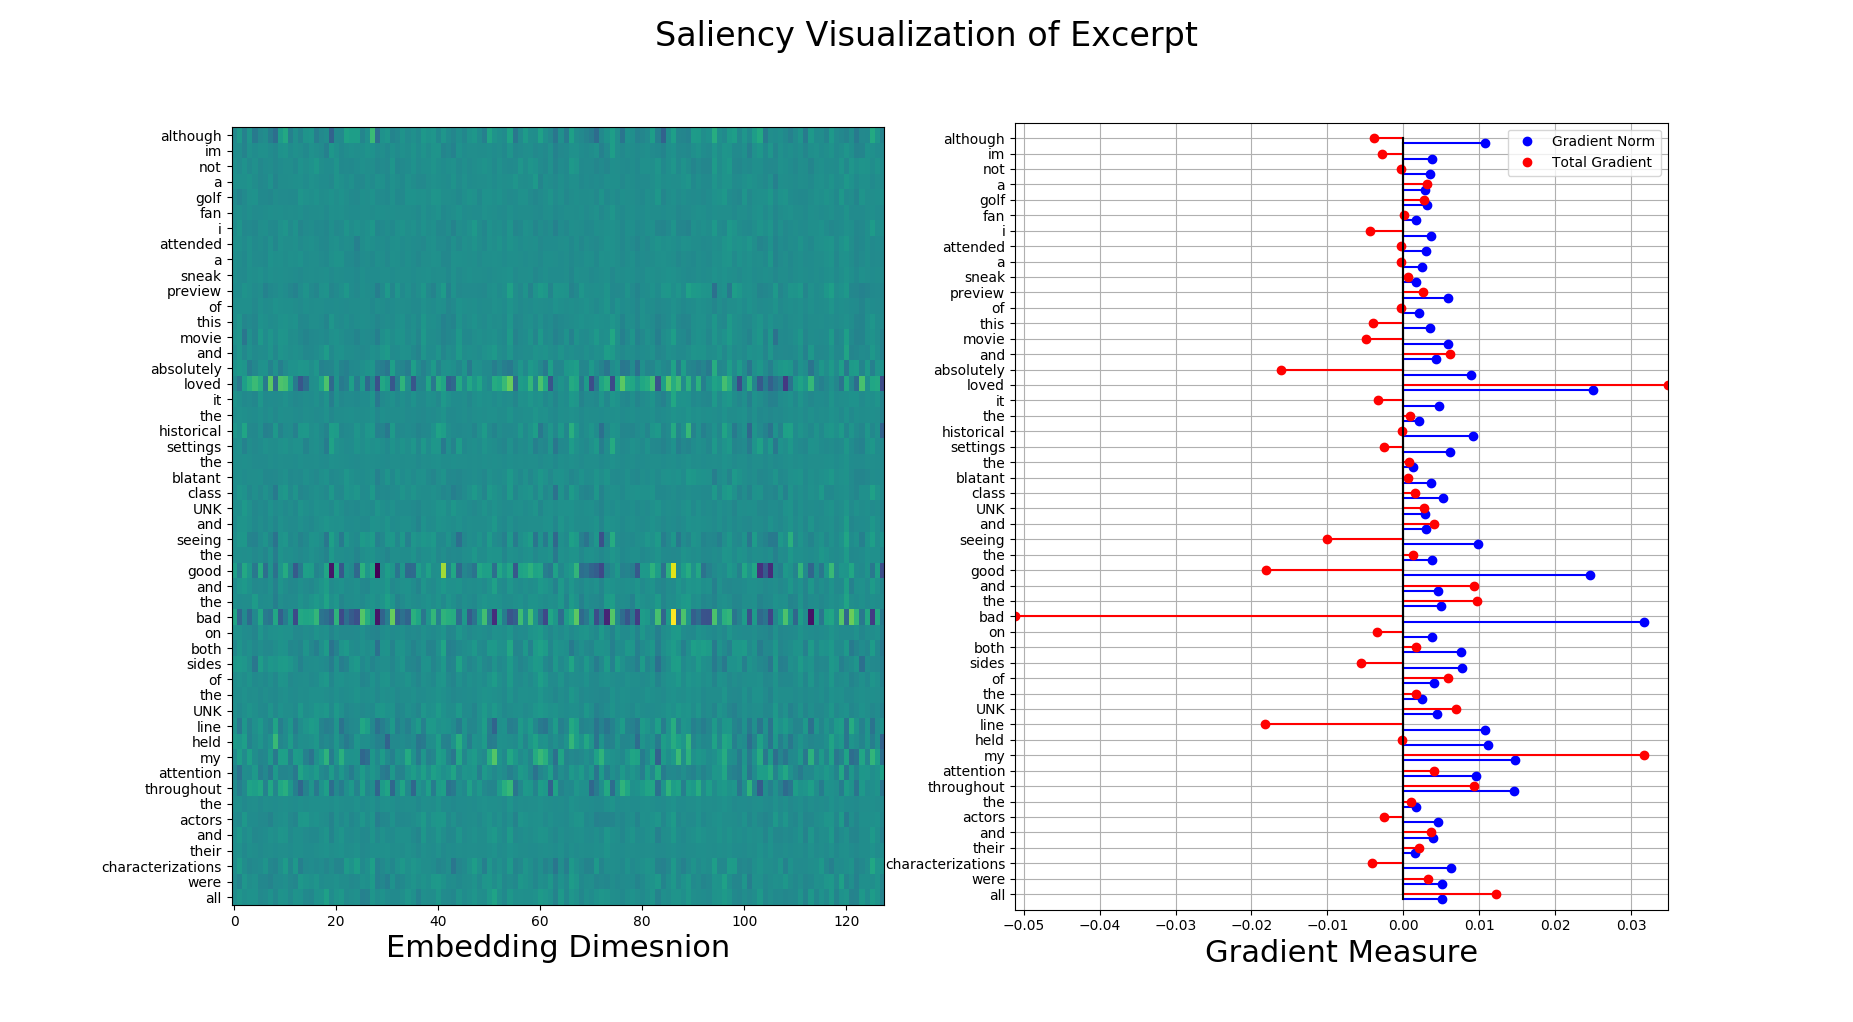
\includegraphics[width=\textwidth]{saliency.png}
    \caption{Different measures of word sentiment/importance}
    \label{fig:saliency}
\end{figure}

In our word embedding, the average value of $\mu$ was $-0.017$, but there was significant variation across embedding dimension.  The average standard deviation was fairly constant over embedding dimension, with a value of $0.55$.  The exact value of the result is not important however.  What this tells us is that words associated with larger gradient norms have a proportionally larger chance of producing an outlier, at least according to the linear approximation.


\chapter{Exponential Windowed Searches}
While gradients overall tend to be useful indicators for small perturbations, they are not entirely useful or accurate in predicting large differences.  This makes sense given that gradient is only a local measure of change.  Since adversarial derivation seeks to find large differences, an algorithm should not rely on the gradient alone.  We discuss three improvements here, each of which builds on the last.  Since it was found that in most cases a classification change could be achieved by replacing only one word, the base strategy focuses on this objective.  If it turns out that more replacements are required, any of the algorithms presented can be extended with an exponential search.

In the case of replacing a single word, the entire search space for a given sample can be described as the Cartesian product of the set of vocabulary words and the set of all sample words.  That is, if $V$ ($|V| = N$) denotes the set of vocabulary words and $S$ ($|S| = M$) denotes the set of sample words (along with their location in the sample), the search space is given by $V\times S$, with the size of the set being $|V\times S| = NM$.  It is convenient to consider sequence equivalents of $V$ and $S$: $v = (v_i)_{i=1}^N$ and $s = (s_i)_{i=1}^M$.  Let a classification function for a sample be given by $r(s)$, and let the sequence $s^{i,j}$ be given by:
\begin{align}\label{eq:replacement_sequence}
s^{i,j} = (s_1,s_2,\dots,s_{i-1},v_j,s_{i+1},\dots,s_M)
\end{align}

\section{Full Search}
For the objective of finding a single adversarial replacement, the brute force solution is simply a full search.  Generate the full matrix: 
\begin{align}\label{eq:class_matrix}
M_{M,N}(\{0,1\}) \ni A_{i,j} = r(s^{i,j})
\end{align}
and search for the symbol that corresponds to an adversarial example.
This method of course has the advantage of achieving the upper bound for performance in generating adversarial derivations with one-word replacements.  It has the disadvantage of being very time intensive.  Assuming the classifier's time complexity is linear in the length of the sample, this algorithm's time complexity is $T=\mathcal{O}(NM^2)$ and its space complexity is $D=\mathcal{O}(W)$, where $W$ is the number of weights stored in the model.

Of course with parallel operations, time complexity can be offloaded to memory complexity as illustrated in Table \ref{tab:fs_complexity}
\begin{table}
\centering
\begin{tabular}{ |c|l|l| } 
 \hline
 Parallelization Tier & Time & Space \\ \hline
 0&$\mathcal{O}(NM^2)$ & $\mathcal{O}(W)$ \\ %\hline
 1&$\mathcal{O}(NM)$ & $\mathcal{O}(WM)$ \\ %\hline
 2&$\mathcal{O}(M^2)$ & $\mathcal{O}(WN)$ \\ %\hline
 3&$\mathcal{O}(M)$ & $\mathcal{O}(WNM)$ \\ \hline
\end{tabular}
\caption{Time and space complexities for full search with varying levels of parallelization.}
\label{tab:fs_complexity}
\end{table}
Note that since the operation of a single recurrent neural network is not parallelizable, the time complexity will always have a factor of at least $M$ no matter how much memory or computing power is available.  With regard to the adversarial matrix $A$, the four complexities above correspond to computing one entry at a time, one row at a time, one column at a time, and computing the entire matrix in parallel, respectively.  

\section{Window Search}
As discussed in the previous section, a full search is not feasible for long samples.  Depending on how the computation is organized, the algorithm will either run out of memory or take far too long to either find a solution or determine that there isn't one.  Looking at the time complexities in Table \ref{tab:fs_complexity}, this is intuitive given that there is a quadratic dependence on $M$, the length of the sample.  As mentioned in section \ref{sec:word_emb_results}, the average length of a review is about 234 words, meaning that typically $M^2 > N$ and sometimes $M^2 \gg N$.  This paper considers two ways to deal with this quadratic growth.

The simplest solution is to cap $M$ at some fixed value, $C$, and discard the rest of the sample.  This method is called cap search.  As discussed in section \ref{sec:rnn_training}, this is in fact an efficient method used to train recurrent neural networks.  Since $V$ and $W$ are also fixed for a given model, this has the advantage of fixing the memory usage in any of the above scenarios.  This is desirable since available memory is a static resource which does not change from iteration to iteration, while time is more flexible.  On the other hand, this method has the obvious drawback that it may either yield an example which is not truly adversarial, or it may fail to find an adversarial example although there is one.  The time and space complexities are given in Table \ref{tab:wa_complexity}.  This search generates the entries of a matrix $A^{cs}$, which we hope is approximately the same as the top $C$ rows of $A$.  Pseudocode is given in Algorithm \ref{alg:cutoff}.

\begin{algorithm}
\begin{algorithmic}[1]
\begin{spacing}{1.0}
    \caption{Simple cutoff algorithm.  Note that this algorithm does not require storage of a matrix as written, but it is convenient for generalization.}
    \Require $s$ \Comment{the sample}
    \Require $r$ \Comment{the classifier function}
    \Require $c$ \Comment{the class obtained}
    \Require $C$ \Comment{the cutoff value}
    \Require $N$ \Comment{the number of words in the vocabulary}
    \State{$S \gets (s_1,s_2,\dots,s_C)$}
    \For{$i = 1$ to $i = C$}
        \For{$j = 1$ to $j = N$}
            \State{$A^{cs}_{i,j} \gets r(S^{i,j})$}
            \If{$A^{cs}_{i,j} \neq c $} 
            \If{$r(s^{i,j}) \neq c$} 
                \State{\Return $s^{i,j}$}
            \EndIf
            \EndIf
        \EndFor
    \EndFor\\
\Return{None}
\label{alg:cutoff}
\end{spacing}
\end{algorithmic}
\end{algorithm}

\begin{table}
\centering
\begin{tabular}{ |c|l|l| } 
 \hline
 Parallelization Tier & Time & Space \\ \hline
 0&$\mathcal{O}(NC^2)$ & $\mathcal{O}(W)$ \\ %\hline
 1&$\mathcal{O}(NC)$ & $\mathcal{O}(WC)$ \\ %\hline
 2&$\mathcal{O}(C^2)$ & $\mathcal{O}(WN)$ \\% \hline
 3&$\mathcal{O}(C)$ & $\mathcal{O}(WNC)$ \\ \hline
\end{tabular}
\caption{Time and space complexities for full search with sample length capped at $C$.}
\label{tab:wa_complexity}
\end{table}

It may be valuable to consider all words in a review for replacement, especially very negative or positive ones.  In this case, the algorithm should still find those words and therefore should consider every word in the sample as a candidate for replacement.  Instead of simply taking the first $C$ words of a sample, take $C$ words surrounding our candidate word, like a sliding window, and infer for every word in the sample.  The new complexities associated with this algorithm are in Table \ref{tab:waw_complexity}.  Since $C$ is strictly less than $M$, this algorithm, called window search (WS), is slower and more memory intensive than the previous algorithm, but should produce more accurate results.  This search generates a matrix $A^{ws}$ which should approximate $A$.  Pseudocode for the algorithm is given in Algorithm \ref{alg:window_search}.

\begin{algorithm}
\begin{algorithmic}[1]
\begin{spacing}{1.0}
    \caption{Window Search algorithm}
    \Require $s$ \Comment{the sample}
    \Require $r$ \Comment{the classifier function}
    \Require $c$ \Comment{the class obtained}
    \Require $C$ \Comment{the window size}
    \Require $N$ \Comment{the number of words in the vocabulary}
    \State{$M \gets \Call{length}{s}$}
    \Function{getWindowSubset}{M,C,n,s}
    \State{$C \gets \Call{min}{C,M}$}
    \State{$n1 \gets n - C//2$}
    \State{$n2 \gets n1 + C - 1$}
    \If{$n1 \geq 1$ and $n2 \leq M$}
            \State{$i1 \gets n1;\text{ } i2 \gets n2$}
        \ElsIf{$n1 < 1$ and $n2 \leq M$}
            \State{$i1 \gets 1;\text{ } i2 \gets C$}
        \ElsIf{$n1 \geq 1$ and $n2 \geq M$}
            \State{$i1 \gets M-C+1;\text{ } i2 \gets M$}
        \Else
            \State{$i1 \gets 1;\text{ } i2 \gets M$}
    \EndIf\\
    \Return $(s_{i1},s_{i1+1},\dots,s_{i2})$
    \EndFunction

    \For{$i = 1$ to $i = M$}
        \State{$S \gets \Call{getWindowSubset}{M,C,i,s}$}
        \For{$j = 1$ to $j = N$}
            \State{$A^{ws}_{i,j} \gets r(S^{i,j})$}
            \If{$A^{cs}_{i,j} \neq c $}
                \If{$r(s^{i,j}) \neq c$} 
                    \State{\Return $s^{i,j}$}
                \EndIf
            \EndIf
        \EndFor
    \EndFor\\
\Return{None}
\label{alg:window_search}
\end{spacing}
\end{algorithmic}
\end{algorithm}

\begin{table}
\centering
\begin{tabular}{ |c|l|l| } 
 \hline
 Parallelization Tier & Time & Space \\ \hline
 0&$\mathcal{O}(NMC)$ & $\mathcal{O}(W)$ \\
 1&$\mathcal{O}(NC)$ & $\mathcal{O}(WM)$ \\
 2&$\mathcal{O}(CM)$ & $\mathcal{O}(WN)$ \\
 3&$\mathcal{O}(C)$ & $\mathcal{O}(WNM)$ \\ \hline
\end{tabular}
\caption{Time and space complexities for window search with a window of size $C$.}
\label{tab:waw_complexity}
\end{table}
\section{Gradient Assisted Window Search}
Finally, the complexity may be reduced even further by using the results of section \ref{sec:stochastic_gradient_analysis}.  Because it was found that words associated with large gradients tend to be good words for replacement, the effective value of $M$ can be reduced in the window search algorithm.  We propose to only consider the top $K$ words for replacement, as ordered by the gradient, and perform a search over those value. This method is called gradient assisted window search (GAWS).  The complexities are given simply by replacing $M$ by $K$ in the window search algorithm, and can be found in Table \ref{tab:gaws_complexity}.  This search generates a matrix $A^{gs}$ which should approximate $K$ rows of $A$ corresponding to the words in the original sample with the $K$ largest gradients.  Pseudocode is given in Algorithm \ref{alg:gaws}.
\begin{algorithm}
\begin{algorithmic}[1]
\begin{spacing}{1.0}
    \caption{Gradient Assisted Window Search (GAWS) algorithm.}
    \Require $s$ \Comment{the sample}
    \Require $r$ \Comment{the classifier function}
    \Require $c$ \Comment{the class obtained}
    \Require $C$ \Comment{the window size}
    \Require $N$ \Comment{the number of words in the vocabulary}
    \State{$M \gets \Call{length}{s}$}
    \For{$i$ in $(1,2,\dots,M)$}
        \State{$g_i \gets ||\nabla r(s_i)||$} \Comment{Get norm of the gradient with respect to the $i^{th}$ input}
    \EndFor
    \State{$I \gets \Call{topInd}{g,K}$} \Comment{Get ordered indices for K largest gradients norms}

    \For{$i$ in $I$}
        \State{$S \gets \Call{getWindowSubset}{M,C,i,s}$} \Comment{See algorithm \ref{alg:window_search} for subroutine}
        \For{$j = 1$ to $j = N$}
            \State{$A^{gs}_{i,j} \gets r(S^{i,j})$}
            \If{$A^{cs}_{i,j} \neq c $}
                \If{$r(s^{i,j}) \neq c$} 
                    \State{\Return $s^{i,j}$}
                \EndIf
            \EndIf
        \EndFor
    \EndFor\\
\Return{None}
\label{alg:gaws}
\end{spacing}
\end{algorithmic}
\end{algorithm}

\begin{table}
\centering
\begin{tabular}{ |c|l|l| } 
 \hline
 Parallelization Tier & Time & Space \\ \hline
 0&$\mathcal{O}(NKC)$ & $\mathcal{O}(W)$ \\
 1&$\mathcal{O}(NC)$ & $\mathcal{O}(WK)$ \\
 2&$\mathcal{O}(CK)$ & $\mathcal{O}(WN)$ \\
 3&$\mathcal{O}(C)$ & $\mathcal{O}(WNK)$ \\ \hline
\end{tabular}
\caption{Time and space complexities for gradient assisted window search with a window of size $C$ and taking the top $K$ words.}
\label{tab:gaws_complexity}
\end{table}
\section{Multi-word Replacement}
Up to this point, only searching for a one-word replacement adversarial derivation has been considered.  While this is sufficient for about $70\%$ of samples, there is still a need to produce derivations for the remaining $30\%$.  Multi-word derivation can be achieved efficiently with two modifications to the original algorithms.

First, instead of dealing with the matrix $A$, one can utilize a more general matrix of classifier confidence levels, rather than just decisions.  Suppose that the function $p(s)$ gives the probability that a sample $s$ is class $0$.  Then in the same way the matrix $A$ is generated along with all of its approximations, the matrix $P_{i,j} = p(s^{i,j})$ can be generated in the same way.  Thresholding this matrix would yield $A$ or its approximation.  Second, if no derivations are detected, one can pick the entry of $P$ with the highest or lowest value (depending on the classification target) and attempt using that substitution.  From this point onward, this work assumes the second tier of parallelization because tier 3 was not feasible on the hardware used in this project.\footnote{All algorithms are run with an AMD RYZEN processor, GTX 1080 Ti GPU, and 32GB of RAM.}

If replacing one word is not successful, the algorithm may select more words.  Doing this naively would lead to combinatorial explosion.  Trying every combination of $L$ words in the full search would cost roughly $\prod_{i=0}^{L-1} (M-i)N = \frac{M!}{(M-L)!}N^L$ lookups, each lookup costing $\mathcal{O}(M)$ time.  Since the time complexity is already a restricting factor, this is not feasible even for small $L$.  We therefore implemented a fast greedy approach where the maximum is taken across all columns of $P$.  This takes $\mathcal{O}(N)$ time and only $\mathcal{O}(M)$ space since the min/max is taken as soon as all elements are available.  The top $L$ entries of the result are chosen as candidate replacements.  Sorting all values in the result requires $\mathcal{O}(M\log(M))$ time.

Now, some method of determining the smallest value of $L$ which allows us to achieve a misclassification is still required.  We assume that replacing more words than required will still lead to a misclassification, and therefore the class vs. $L$ curve looks like a step function.  Since it is monotonic, we can use an exponential search for the transition point which runs in $\mathcal{O}(M\log L)$ time and $\mathcal{O}(W+M)$ space given that all candidates have already been determined.  This will usually be better than a binary search given that the number of words being replaced, $L$ is often small compared to the size of the sample, $M$.  Adding all steps together, the final time and space complexities of the given algorithms can be found in Table \ref{tab:overall_complexity}.

In order to obtain the modified pseudocode for Algorithm \ref{alg:window_search}, replace lines 20 to 25 with $P^{ws}_{i,j} \gets p(S^{i,j})$ and append Algorithm \ref{alg:exp}.  Algorithm \ref{alg:gaws} can be extended in the same way, except by replacing lines 9 to 14. 

\begin{algorithm}
\begin{algorithmic}[1]
\begin{spacing}{1.0}
    \caption{Exponential Search Algorithm for Multi-word Replacement}
    \Require $s$ \Comment{the sample}
    \Require $r$ \Comment{the classifier function}
    \Require $c$ \Comment{the class obtained}
    \Require $P$ \Comment{probability matrix}
    \State{$L \gets \Call{length}{s}$}
    \For{$i=1$ to $i=L$}
        \If{c = 0}
        \State{$p_i \gets \Call{min}{P_i}$; $I_i \gets \Call{argmin}{P_i}$}\Comment{$P_i$ is the $i^{th}$ row of $P$}
        \ElsIf{c = 1}
        \State{$p_i \gets \Call{max}{P_i}$; $I_i \gets \Call{argmax}{P_i}$}
        \EndIf
        \State{$J_i \gets i$}
    \EndFor\\
    \State{$L \gets 0$; $R \gets 1$}
    \While{$L < R$}
        \If{$LimitFound = False$}
            \State{$R \gets 2\times R$}
        \EndIf
        \State{$m \gets (L + R) // 2$}
        \If{$c = 1$}
            \State{$args \gets \Call{topInd}{p,m}$}\Comment{get arguments of largest probabilities}
        \ElsIf{$c = 1$}
            \State{$args \gets \Call{botInd}{p,m}$}\Comment{get arguments of smallest probabilities}
        \EndIf
        \State{$Is \gets I[args]$; $Js \gets J[args]$ }
        \State{$S \gets s$} 
        \For{$i = 1$ to $m$}
            \State{$S_{Js_i} \gets D_{Is_i}$} \Comment{$D$ is the dictionary of all words}
        \EndFor
        \If{$r(S) = c$ and $limitFound = True$}
            \State{$L \gets m + 1$}
        \ElsIf{$r(S) \neq c$}
            \State{$limitFound \gets True$}
            \State{$R \gets m - 1$}
            \State{$minm \gets \Call{min}{minm,m}$}
            \If{$m = minm$}
                \State{$bestS \gets S$}
            \EndIf
        \EndIf
    \EndWhile\\
\If{$limitFound = True$}
\State{\Return{$bestS$}}
\EndIf\\
\Return{None}
\label{alg:exp}
\end{spacing}
\end{algorithmic}
\end{algorithm}

\begin{table}
\centering
\begin{tabular}{ |c|c|c| } 
 \hline
 Method & Time & Space \\ \hline
 Full Search & $\mathcal{O}(M^2 + M\log(M) + M\log L)$ & $\mathcal{O}(WN)$ \\ \hline 
 Cap Search & $\mathcal{O}(C^2 + C\log(C) + M\log L)$ & $\mathcal{O}(WN)$ \\ \hline 
 Window Search & $\mathcal{O}(CM + M\log(M) + M\log L)$ & $\mathcal{O}(WN)$ \\ \hline 
 GAWS & $\mathcal{O}(CK + K\log(K) + M\log L)$ & $\mathcal{O}(WN)$ \\ \hline 
\end{tabular}
\caption{Overall time complexities for several search algorithms extended with an exponential search for multi-word replacement.  These complexities assume the second tier of parallelization found in tables \ref{tab:fs_complexity} through \ref{tab:gaws_complexity}.}
\label{tab:overall_complexity}
\end{table}

\chapter{Results}
In our preliminary examination of the data, we saw that a sample which was very confidently and correctly labeled as positive, could be confidently mislabeled by switching only a single word with another.  If we are attempting to generate discrete adversarial examples, we may simply attempt replacing every word in the sample with every possible word in the vocabulary.  The number of classifications would then be $V\times N$ which is of course very large and therefore even replacing one word is time consuming.  If it turns out we must replace $m>1$ words, this task requires 
\begin{equation}
N(m) = (V\times N)(V\times (N-1))\dots(V\times (N-m)) = \frac{V^m N!}{(N-m)!}
\end{equation}
classifications making it an intractable problem.

Using the approximated delta to determine good candidate words for switching resulted in relatively poor results, with the largest values giving only modest actual changes in prediction confidence.  Instead of determining pairs of words to swap directly, we use measures of the gradient to determine the top candidate words in the text sample and swap them with every other word in the vocabulary.  If we search the words with the top $k$ gradient norms, then replacing $m$ words requires
\begin{equation}
N(m) = (V\times k)^m
\end{equation}
classifications.  This method is still untractable for even modest $m$ since the vocabulary is so large.  However, as discussed in chapter \ref{}, empirical results for our classification architecture and data set that at least 73.3\% of samples correctly labeled by our architecture can be altered by just one word and then mislabeled.

\section{White Box}
All details of model known, algorithm run directly on model.
\section{Gray Box}
General structure of model known including hyperparameters
 algorithm run on stand-in model trained on same data, but not same model.
\section{Black Box}
Model is completely unknown, hyperparameters vary from stand-in model.


\chapter{Conclusion}
-x-
\section{Discussion}
-x-
\section{Future Work}
More complex neural networks
Reduce difference between source word and destination word

\bibliography{references}{}
\appendix
\chapter{Code Appendix}
This appendix includes a large sample of code used to obtain the results displayed in this thesis.  Code should not be used without understanding, as certain programs may be used as a template rather than a standalone module.

\end{document}
\grid
